\documentclass[hyperref,dvipsnames,svgnames,compress]{beamer}

\usepackage{amsmath, tikz, subfigure, graphicx}
\usepackage{multirow,colortbl}
\usepackage[customcolors,norndcorners]{hf-tikz}

\usetikzlibrary{decorations.pathreplacing,decorations.pathmorphing,arrows,positioning,shapes,shapes.multipart}

\title[Approximation Algorithms for FTFP]{Approximation Algorithms
  for the Fault-Tolerant Facility Placement Problem}
\author[lyan@cs.ucr.edu]{Li Yan}
\institute[UCR]{
  Computer Science\\
  University of California Riverside\\
}
\date{06/10/2013}
\usetheme{Warsaw}

\AtBeginSection[]
{
  \begin{frame}{Table of Contents}
    \tableofcontents[currentsection,hideallsubsections,subsubsectionstyle=hide]
  \end{frame}
}


\defbeamertemplate*{footline}{shadow theme}
{%
  \leavevmode%
  \hbox{\begin{beamercolorbox}[wd=.5\paperwidth,ht=2.5ex,dp=1.125ex,leftskip=.3cm plus1fil,rightskip=.3cm]{author in head/foot}%
    \usebeamerfont{author in head/foot}\insertframenumber\,/\,\inserttotalframenumber\hfill\insertshortauthor
  \end{beamercolorbox}%
  \begin{beamercolorbox}[wd=.5\paperwidth,ht=2.5ex,dp=1.125ex,leftskip=.3cm,rightskip=.3cm plus1fil]{title in head/foot}%
    \usebeamerfont{title in head/foot}\insertshorttitle%
  \end{beamercolorbox}}%
  \vskip0pt%
}


%%%%%%%%%%%%%%%%%%%%%%%%%%%%%%%%%%%%%%%%%%%%%%%%%%%%%%%%%%

% non-math stuff

\newcommand{\myparagraph}[1]{{\medskip\noindent{\bf #1}}}
\newcommand{\emparagraph}[1]{{\medskip\noindent{\it #1}}}
\newcommand{\etal}{{\it et al.}}
\newcommand{\myif}{{\mbox{\rm\ if \ }}}
\newcommand{\mycase}[1]{\mbox{{\underline{Case #1}}:\/}}

\newcommand{\margincomment}[1]%
    {{%
      \marginpar{{\tiny\begin{minipage}{0.5in}
                       \begin{flushleft}
                          {#1}
                       \end{flushleft}
                       \end{minipage}
                }}
    }}


%%%%%%%%%%%%%%%%%%%%%%%%%%%%%%%%%%%%%%%%%%%%%%%%%%%%%%%%%%

% various letters

\newcommand{\hatc}{{\hat c}}
\newcommand{\hatC}{{\hat C}}
\newcommand{\hatr}{{\hat r}}
\newcommand{\hatx}{{\hat x}}
\newcommand{\haty}{{\hat y}}
\newcommand{\dotx}{{\dot x}}
\newcommand{\doty}{{\dot y}}
\newcommand{\dotr}{{\dot r}}
\newcommand{\boldx}{{\mathbf x}}

\newcommand{\doubledone}{{\bar 1}}
\newcommand{\doubledtwo}{{\bar 2}}
\newcommand{\barc}{{\bar c}}
\newcommand{\bart}{{\bar t}}

\newcommand{\barx}{{\bar x}}
\newcommand{\bary}{{\bar y}}
\newcommand{\barz}{{\bar z}}
\newcommand{\barr}{{\bar r}}
\newcommand{\barX}{{\bar X}}
\newcommand{\barY}{{\bar Y}}
\newcommand{\barZ}{{\bar Z}}
\newcommand{\bara}{{\bar a}}
\newcommand{\bard}{{\bar d}}
\newcommand{\barm}{{\bar m}}
\newcommand{\barA}{{\bar A}}
\newcommand{\barB}{{\bar B}}
\newcommand{\barC}{{\bar C}}
\newcommand{\barG}{{\bar G}}
\newcommand{\barE}{{\bar E}}
\newcommand{\barV}{{\bar V}}

\newcommand{\wbarC}{{\overline{C}}}
\newcommand{\wbarD}{{\overline{D}}}
\newcommand{\wbarN}{{\overline{N}}}
\newcommand{\wbarX}{{\overline{X}}}


\newcommand{\barbeta}{{\bar\beta}}
\newcommand{\bargamma}{{\bar\gamma}}
\newcommand{\apomega}{{\bar\omega}}

\newcommand{\bfr}{\boldsymbol{r}}
\newcommand{\bfv}{{\bf v}}
\newcommand{\bfx}{\boldsymbol{x}}
\newcommand{\bfy}{\boldsymbol{y}}
\newcommand{\bfz}{{\bf z}}
\newcommand{\bfQ}{{\bf Q}}
\newcommand{\bfR}{{\bf R}}
\newcommand{\bfS}{{\bf S}}
\newcommand{\bfT}{{\bf T}}
\newcommand{\bfV}{{\bf V}}
\newcommand{\bfone}{{\bf 1}}
\newcommand{\bfalpha}{\boldsymbol{\alpha}}
\newcommand{\bfbeta}{\boldsymbol{\beta}}

\newcommand{\calA}{{\cal A}}
\newcommand{\calB}{{\cal B}}
\newcommand{\calC}{{\cal C}}
\newcommand{\calD}{{\cal D}}
\newcommand{\calE}{{\cal E}}
\newcommand{\calG}{{\cal G}}
\newcommand{\calH}{{\cal H}}
\newcommand{\calJ}{{\cal J}}
\newcommand{\calK}{{\cal K}}
\newcommand{\calL}{{\cal L}}
\newcommand{\calM}{{\cal M}}
\newcommand{\calN}{{\cal N}}
\newcommand{\calS}{{\cal S}}
\newcommand{\calU}{{\cal U}}
\newcommand{\calX}{{\cal X}}
\newcommand{\calT}{{\cal T}}

\newcommand{\hatcalI}{{\hat{\cal I}}}
\newcommand{\barcalI}{{\bar{\cal I}}}
\newcommand{\dotcalI}{{\dot{\cal I}}}

\newcommand{\vecS}{{\bar S}}
\newcommand{\vecT}{{\bar T}}
\newcommand{\vecone}{{\bf 1}}
\newcommand{\tildec}{{\tilde c}}
\newcommand{\tilded}{{\tilde d}}
\newcommand{\tildeD}{{\tilde D}}
\newcommand{\tildeC}{{\widetilde C}}
\newcommand{\tildeZ}{{\tilde Z}}
\newcommand{\tilder}{{\widetilde r}}
\newcommand{\tildex}{{\widetilde x}}
\newcommand{\wtildeN}{{\widetilde N}}
\newcommand{\tildebfr}{\widetilde{\boldsymbol{r}}}
\newcommand{\tildebfx}{\widetilde{\boldsymbol{x}}}
\newcommand{\tildebfy}{\widetilde{\boldsymbol{y}}}

\newcommand{\barbfx}{\bar{\boldsymbol{x}}}
\newcommand{\barbfy}{\bar{\boldsymbol{y}}}
\newcommand{\hatbfx}{\hat{\boldsymbol{x}}}
\newcommand{\hatbfy}{\hat{\boldsymbol{y}}}
\newcommand{\dotbfx}{\dot{\boldsymbol{x}}}
\newcommand{\dotbfy}{\dot{\boldsymbol{y}}}

\newcommand{\wbarcalC}{{\overline{\calC}}}
\newcommand{\wbarcalD}{{\overline{\calD}}}
\newcommand{\eps}{{\epsilon}}

%%%%%%%%%%%%%%%%%%%%%%%%%%%%%%%%%%%%%%%%%%%%%%%%%%%%%%%%%%

\newcommand{\half}{{\mbox{$\frac{1}{2}$}}}
\newcommand{\threehalfs}{{\mbox{$\frac{3}{2}$}}}
\newcommand{\threefourths}{{\mbox{$\frac{3}{4}$}}}
\newcommand{\fivehalfs}{{\mbox{$\frac{5}{2}$}}}
\newcommand{\onethird}{{\mbox{$\frac{1}{3}$}}}
\newcommand{\twothirds}{{\mbox{$\frac{2}{3}$}}}
\newcommand{\fourthirds}{{\mbox{$\frac{4}{3}$}}}
\newcommand{\fivethirds}{{\mbox{$\frac{5}{3}$}}}
\newcommand{\fivefourths}{{\mbox{$\frac{5}{4}$}}}
\newcommand{\onefourth}{{\mbox{$\frac{1}{4}$}}}
\newcommand{\onefifth}{{\mbox{$\frac{1}{5}$}}}
\newcommand{\twofifths}{{\mbox{$\frac{2}{5}$}}}
\newcommand{\threefifths}{{\mbox{$\frac{3}{5}$}}}
\newcommand{\fourfifths}{{\mbox{$\frac{4}{5}$}}}
\newcommand{\ninefifths}{{\mbox{$\frac{9}{5}$}}}
\newcommand{\sevensixths}{{\mbox{$\frac{7}{6}$}}}
\newcommand{\oneeighth}{{\mbox{$\frac{1}{8}$}}}
\newcommand{\threeeighths}{{\mbox{$\frac{3}{8}$}}}
\newcommand{\fiveeighths}{{\mbox{$\frac{5}{8}$}}}
\newcommand{\seveneighths}{{\mbox{$\frac{7}{8}$}}}
\newcommand{\onetenth}{{\mbox{$\frac{1}{10}$}}}
\newcommand{\seventenths}{{\mbox{$\frac{7}{10}$}}}
\newcommand{\ninetenths}{{\mbox{$\frac{9}{10}$}}}
\newcommand{\twonineths}{{\mbox{$\frac{2}{9}$}}}
\newcommand{\fivenineths}{{\mbox{$\frac{5}{9}$}}}
\newcommand{\elevennineths}{{\mbox{$\frac{11}{9}$}}}
\newcommand{\threetwentieths}{{\mbox{$\frac{3}{20}$}}}
\newcommand{\twentyfivenineteenths}{{\mbox{$\frac{25}{19}$}}}

\newcommand{\sqrttwo}{\sqrt{2}}

%%%%%%%%%%%%%%%%%%%%%%%%%%%%%%%%%%%%%%%%%%%%%%%%%%%%%%%%%%

% various delimiters

\newcommand{\braced}[1]{{ \left\{ #1 \right\} }}
\newcommand{\angled}[1]{{ \left\langle #1 \right\rangle }}
\newcommand{\brackd}[1]{{ \left[ #1 \right] }}
\newcommand{\parend}[1]{{ \left( #1 \right) }}
\newcommand{\barred}[1]{{ \left| #1 \right| }}
\newcommand{\dbarred}[1]{{ \left\| #1 \right\| }}
\newcommand{\floor}[1]{{ \lfloor #1 \rfloor }}
\newcommand{\ceiling}[1]{{ \lceil #1 \rceil }}

%%%%%%%%%%%%%%%%%%%%%%%%%%%%%%%%%%%%%%%%%%%%%%%%%%%%%%%%%%

% some math symbols

\newcommand{\set}{\,{\leftarrow}\,}
\newcommand{\suchthat}{{\,:\,}}
\newcommand{\cost}{{\it cost}}
\newcommand{\yield}{{\it yield}}
\newcommand{\opt}{{\it opt}}

\newcommand{\algA}{{\bf A}}
\newcommand{\LHS}{{\rm LHS}}
\newcommand{\RHS}{{\rm RHS}}
\newcommand{\reals}{{\bf R}}
\newcommand{\posreals}{{\bf R}^+}

\newcommand{\assign}{{\,\leftarrow\,}}

\newcommand{\absvalue}[1]{{\barred{#1}}}
\newcommand{\posvalue}[1]{{\brackd{#1}^+}}

\newcommand{\NP}{{\mbox{\sf NP}}}
\newcommand{\PP}{{\mbox{\sf P}}}
\newcommand{\DTIME}{{\mbox{\sf DTIME}}}

\newcommand{\letbox}[1]{{\makebox[11pt]{{\small {$#1$}}}}}
\newcommand{\optstring}[1]{{ \frame{\;\raisebox{0pt}[12pt][5pt]{#1}\;} }}

\newcommand{\leftend}{{\diamond}}
\newcommand{\rightend}{{\diamond}}

%\newcommand{\argmin}{{\mbox{\rm argmin}}}
\DeclareMathOperator*{\argmin}{arg\,min}

\newcommand\litem[1]{\item{\bfseries #1\enspace}}
\newcommand{\ceil}[1] {\lceil #1 \rceil}
\newcommand{\naive}{na\"{\i}ve}
\newcommand{\LP}{\mbox{\rm LP}}
\newcommand{\OPT}{\mbox{\rm OPT}}
\newcommand{\ALG}{\mbox{\rm ALG}}
\newcommand{\LPR}[1]{{\mbox{\rm LPR#1}}}
\newcommand{\smallLPR}[1]{{\mbox{\tiny\rm LPR#1}}}
% algorithm names
\newcommand{\ESTA}{\mbox{\rm ESTA}} % 4approx
\newcommand{\EGUP}{\mbox{\rm EGUP}} % 3approx
\newcommand{\ECHS}{\mbox{\rm ECHS}} % 1.736
\newcommand{\EBGS}{\mbox{\rm EBGS}} % 1.575
\newcommand{\GUP}{\mbox{\rm GUP}}
\newcommand{\smallESTA}{\mbox{\tiny\rm ESTA}}
\newcommand{\smallEGUP}{\mbox{\tiny\rm EGUP}}
\newcommand{\smallECHS}{\mbox{\tiny\rm ECHS}}
\newcommand{\smallEBGS}{\mbox{\tiny\rm EBGS}}

\newcommand{\SOL}[1]{{{\mbox{\rm SOL}}_{#1}}}
\newcommand{\FTFP}{\mbox{\rm FTFP}}
\newcommand{\FTFL}{\mbox{\rm FTFL}}
\newcommand{\calI}{\mathcal{I}}
\newcommand{\avg}{{\mbox{\scriptsize\rm avg}}}

\newcommand{\dmax}{\text{dmax}}
\newcommand{\davg}{\text{davg}}
\newcommand{\favg}{f_{\text{avg}}}
\newcommand{\conn}{\text{conn}}
\newcommand{\cls}{\text{cls}}
\newcommand{\far}{\text{far}}

\newcommand{\sitesset}{\mathbb{F}}
\newcommand{\clientset}{\mathbb{C}}
\newcommand{\facilityset}{\overline{\sitesset}}
\newcommand{\demandset}{\overline{\clientset}}

%\newcommand{\dist}{{\mbox{dist}}}
\newcommand{\concost}{C^{\avg}}
\newcommand{\faccost}{F^{\avg}}
\newcommand{\tcc}{\mbox{\rm{tcc}}}
\newcommand{\clsdist}{C_{\cls}^{\avg}}
\newcommand{\fardist}{C_{\far}^{\avg}}
\newcommand{\clsmax}{C_{\cls}^{\max}}
\newcommand{\clsnb}{N_{\cls}}
\newcommand{\farnb}{N_{\far}}
\newcommand{\wbarclsnb}{\wbarN_{\cls}}
\newcommand{\wbarfarnb}{\wbarN_{\far}}
\newcommand{\wtildeclsnb}{\wtildeN_{\cls}}
\newcommand{\tcccls}{\mbox{\rm{tcc}}_{\cls}}
\newcommand{\dmaxcls}{\mbox{\rm{dmax}}_{\cls}}

\newcommand{\Exp}{\mbox{\rm Exp}}

\newcommand{\FacilityDistSort}{{\textsc{FacilityDistSort}}}
\newcommand{\NearestUnitChunk}{{\textsc{NearestUnitChunk}}}
\newcommand{\AugmentToUnit}{{\textsc{AugmentToUnit}}}
\newcommand{\connsum}{{\textrm{conn}}}

%%%%%%%%%%%%%%%%%%%%%%%%%%%%%%%%%%%%%%%%%%%%%%%%%%%%%%%%%%

% theorem and such

\newtheorem{theorem}{Theorem}
\newtheorem{definition}[theorem]{Definition}
\newtheorem{corollary}[theorem]{Corollary}
\newtheorem{lemma}[theorem]{Lemma}
\newtheorem{fact}[theorem]{Fact}
\newtheorem{claim}[theorem]{Claim}
\newtheorem{conjecture}[theorem]{Conjecture}
\newtheorem{observation}[theorem]{Observation}

%%%%%%%%%%%%%%%%%%%%%%%%%%%%%%%%%%%%%%%%%%%%%%%%%%%%%%%%%%

\newcommand{\ignore}[1]{}

\definecolor{light-gray}{gray}{0.7}
\begin{document}
%% (5-10min)  1. What is the problem: motivation, definition, related work
%% (5-10min)  2. What results do you have: approximation ratio
%% (30-40min) 3. How did you solve it: techniques
%% (5min)     4. How to improve it: open problems, future work
%%%
\begin{frame}
  \titlepage
\end{frame}

%%%%%%%%%%%%%%%%%%%%%%%%%%%%%%%%%%%%%%%%%%%%%%%%%%%%
%%% outline
%%%%%%%%%%%%%%%%%%%%%%%%%%%%%%%%%%%%%%%%%%%%%%%%%%%%
\begin{frame}
  \frametitle{Outline}
  \tableofcontents[hideallsubsections]
\end{frame}

%% 1. What is the problem: motivation, definition, related work
%% - motivation: ISP/residents, data center/consumer
%% - definition: F, C, r_j, d_ij, f_i, what is a solution and what is the cost
%% - related work: UFL and FTFL
%%% problem example
%%% instance with annotation

%%%%%%%%%%%%%%%%%%%%%%%%%%%%%%%%%%%%%%%%%%%%%%%%%
%% The FTFP problem definition
%%%%%%%%%%%%%%%%%%%%%%%%%%%%%%%%%%%%%%%%%%%%%%%%%
\section[FTFP]{The FTFP Problem}
\begin{frame}
  \frametitle{Fault-Tolerant Facility Placement Problem (FTFP)}
  \setbeamercovered{invisible}
  \begin{center}
  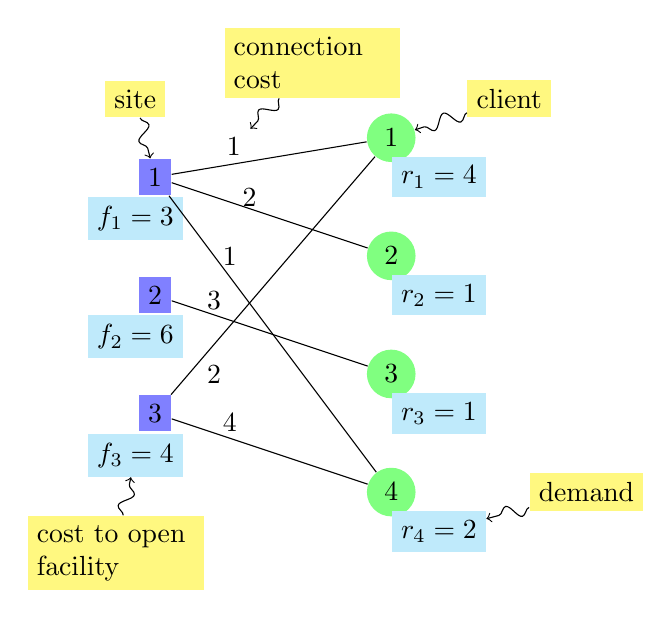
\begin{tikzpicture}[scale=0.5,decoration=snake]
    \node[fill=blue!50] (fac3) at (0,2) {$3$};
    \node[fill=blue!50] (fac2) at (0,5) {$2$};
    \node[fill=blue!50] (fac1) at (0,8) {$1$};

    \node[below,fill=cyan!25] (faclabel3) at (-.5,1.5) {$f_3=4$};
    \node[below,fill=cyan!25] (faclabel2) at (-.5,4.5) {$f_2=6$};
    \node[below,fill=cyan!25] (faclabel1) at (-.5,7.5) {$f_1=3$};

    \node[circle,fill=green!50] (client4) at (6,0) {$4$};
    \node[circle,fill=green!50] (client3) at (6,3) {$3$};
    \node[circle,fill=green!50] (client2) at (6,6) {$2$};
    \node[circle,fill=green!50] (client1) at (6,9) {$1$};

    \node[right,fill=cyan!25] (demand4) at (6,-1) {$r_4=2$};
    \node[right,fill=cyan!25] (demand3) at (6,2) {$r_3=1$};
    \node[right,fill=cyan!25] (demand2) at (6,5) {$r_2=1$};
    \node[right,fill=cyan!25] (demand1) at (6,8) {$r_1=4$};

    \foreach \from/\to in {fac3/client4,fac3/client1,fac2/client3,fac1/client4,fac1/client2,fac1/client1}
    \draw (\from)--(\to);

    % edge weight
    \node[above] (ew11) at (2,8.3) {$1$};
    \node[above] (ew12) at (2.4,7) {$2$};
    \node[above] (ew14) at (1.9,5.5) {$1$};
    \node[above] (ew23) at (1.5,4.4) {$3$};
    \node[above] (ew33) at (1.5,2.5) {$2$};
    \node[above] (ew34) at (1.9,1.3) {$4$};


    \pause
    % annotations
    \node[above,fill=yellow!50] (sites) at (-.5,9.5) {site}; 
    \draw[->,decorate] (sites) -- (fac1);

    \node[above,fill=yellow!50] (clients) at (9,9.5) {client};
    \draw[->,decorate] (clients) -- (client1);

    \node[right,fill=yellow!50] (demand) at (9.5,0) {demand};
    \draw[->,decorate] (demand) -- (demand4);

    \node[above,fill=yellow!50,text width=2cm] (fi) at (-1,-2.5) {cost to open facility};
    \draw[->,decorate] (fi) -- (faclabel3);

    \node[above,fill=yellow!50,text width=2cm] (edge) at (4,10) {connection cost};
    \draw[->,decorate] (edge) -- (ew11);
  \end{tikzpicture}
  \end{center}
\end{frame}

\begin{frame}
  \frametitle{Fault-Tolerant Facility Placement Problem (FTFP)}

  \begin{center}
  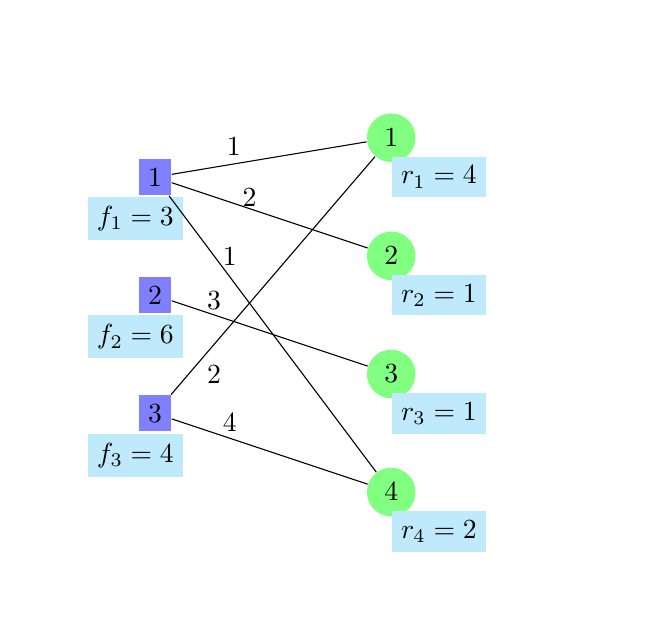
\begin{tikzpicture}[scale=0.5,decoration=snake]
    \node[fill=blue!50] (fac3) at (0,2) {$3$};
    \node[fill=blue!50] (fac2) at (0,5) {$2$};
    \node[fill=blue!50] (fac1) at (0,8) {$1$};

    \node[below,fill=cyan!25] (faclabel3) at (-.5,1.5) {$f_3=4$};
    \node[below,fill=cyan!25] (faclabel2) at (-.5,4.5) {$f_2=6$};
    \node[below,fill=cyan!25] (faclabel1) at (-.5,7.5) {$f_1=3$};

    \node[circle,fill=green!50] (client4) at (6,0) {$4$};
    \node[circle,fill=green!50] (client3) at (6,3) {$3$};
    \node[circle,fill=green!50] (client2) at (6,6) {$2$};
    \node[circle,fill=green!50] (client1) at (6,9) {$1$};

    \node[right,fill=cyan!25] (demand4) at (6,-1) {$r_4=2$};
    \node[right,fill=cyan!25] (demand3) at (6,2) {$r_3=1$};
    \node[right,fill=cyan!25] (demand2) at (6,5) {$r_2=1$};
    \node[right,fill=cyan!25] (demand1) at (6,8) {$r_1=4$};
    
    \foreach \from/\to in {fac3/client4,fac3/client1,fac2/client3,fac1/client4,fac1/client2,fac1/client1}
    \draw (\from)--(\to);

    % edge weight
    \node[above] (ew11) at (2,8.3) {$1$};
    \node[above] (ew12) at (2.4,7) {$2$};
    \node[above] (ew14) at (1.9,5.5) {$1$};
    \node[above] (ew23) at (1.5,4.4) {$3$};
    \node[above] (ew33) at (1.5,2.5) {$2$};
    \node[above] (ew34) at (1.9,1.3) {$4$};

    % remove annotations, use white, ugly solution
    \node[above,fill=white,color=white] (sites) at (-.5,9.5) {site}; 
    \draw[->,decorate,draw=none] (sites) -- (fac1);

    \node[above,fill=white,color=white] (clients) at (9,9.5) {client};
    \draw[->,decorate,draw=none] (clients) -- (client1);

    \node[right,fill=white,color=white] (demand) at (9.5,0) {demand};
    \draw[->,decorate,draw=none] (demand) -- (demand4);

    \node[above,fill=white,color=white,text width=2cm] (fi) at (-1,-2.5) {cost to open facility};
    \draw[->,decorate,draw=none] (fi) -- (faclabel3);

    \node[above,fill=white,color=white,text width=2cm] (edge) at (4,10) {connection cost};
    \draw[->,decorate,draw=none] (edge) -- (ew11);

  \end{tikzpicture}
  \end{center}
\end{frame}

%%% A feasible solution
\begin{frame}
  \frametitle{Feasible Integral Solution}
  \begin{columns}
    \column{0.5\textwidth}
    \begin{figure}[ht]
      \begin{center}
      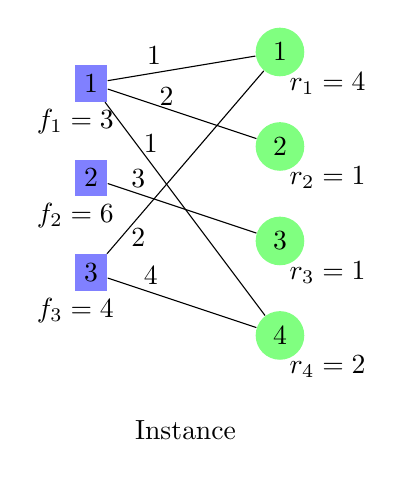
\begin{tikzpicture}[scale=0.4]
        \node[fill=blue!50] (fac3) at (0,2) {$3$};
        \node[fill=blue!50] (fac2) at (0,5) {$2$};
        \node[fill=blue!50] (fac1) at (0,8) {$1$};

        \node[below] (faclabel3) at (-.5,1.5) {$f_3=4$};
        \node[below] (faclabel2) at (-.5,4.5) {$f_2=6$};
        \node[below] (faclabel1) at (-.5,7.5) {$f_1=3$};

        \node[circle,fill=green!50] (client4) at (6,0) {$4$};
        \node[circle,fill=green!50] (client3) at (6,3) {$3$};
        \node[circle,fill=green!50] (client2) at (6,6) {$2$};
        \node[circle,fill=green!50] (client1) at (6,9) {$1$};

        \node[right] (demand4) at (6,-1) {$r_4=2$};
        \node[right] (demand3) at (6,2) {$r_3=1$};
        \node[right] (demand2) at (6,5) {$r_2=1$};
        \node[right] (demand1) at (6,8) {$r_1=4$};
    
        \foreach \from/\to in {fac3/client4,fac3/client1,fac2/client3,fac1/client4,fac1/client2,fac1/client1}
        \draw (\from)--(\to);

        % edge weight
        \node[above] (ew11) at (2,8.3) {$1$};
        \node[above] (ew12) at (2.4,7) {$2$};
        \node[above] (ew14) at (1.9,5.5) {$1$};
        \node[above] (ew23) at (1.5,4.4) {$3$};
        \node[above] (ew33) at (1.5,2.5) {$2$};
        \node[above] (ew34) at (1.9,1.3) {$4$};

        \node (label1) at (3,-3) {Instance};
      \end{tikzpicture}
    \end{center}
  \end{figure}

  \column<2->{0.5\textwidth}
  \begin{figure}[ht]
    \begin{center}
    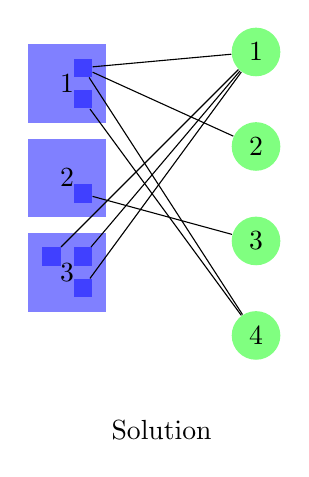
\begin{tikzpicture}[scale=0.4]
      \node[fill=blue!50,minimum size=1cm] (fac3) at (0,2) {$3$};
      \node[fill=blue!75,minimum size=.2cm] (fac33) at (.5,1.5) {};
      \node[fill=blue!75,minimum size=.2cm] (fac32) at (.5,2.5) {};
      \node[fill=blue!75,minimum size=.2cm] (fac31) at (-.5,2.5) {};

      \node[fill=blue!50,minimum size=1cm] (fac2) at (0,5) {$2$};
      \node[fill=blue!75,minimum size=.2cm] (fac21) at (.5,4.5) {};

      \node[fill=blue!50,minimum size=1cm] (fac1) at (0,8) {$1$};
      \node[fill=blue!75,minimum size=.2cm] (fac12) at (.5,7.5) {};
      \node[fill=blue!75,minimum size=.2cm] (fac11) at (.5,8.5) {};

      \node[circle,fill=green!50] (client4) at (6,0) {$4$};
      \node[circle,fill=green!50] (client3) at (6,3) {$3$};
      \node[circle,fill=green!50] (client2) at (6,6) {$2$};
      \node[circle,fill=green!50] (client1) at (6,9) {$1$};
    
      \foreach \from/\to in {fac31/client1,fac32/client1,fac33/client1,fac11/client1,fac11/client2,fac11/client4,fac21/client3,fac12/client4}
      \draw (\from)--(\to);
    
      \node (label1) at (3,-3) {Solution};
  \end{tikzpicture}
    \end{center}
  \end{figure}
  %
  \end{columns}

  \begin{block}<3->{Cost}
    $2f_1 + f_2 + 3f_3 + d_{11} + d_{12} + 2d_{14} +
  d_{23} + 3d_{31} = 38$
  \end{block}
  %

  % cost
\end{frame}

\begin{frame}
  \frametitle{Metric Distances: Triangle Inequality}
  \begin{columns}
    \column{0.5\textwidth}  %% picture for triangle inequality
    \begin{center}
      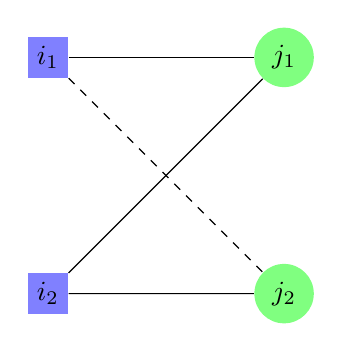
\begin{tikzpicture}[scale=.6]
        \node[fill=blue!50] (fac1) at (0,0) {$i_1$};
        \node[fill=blue!50] (fac2) at (0,-5) {$i_2$};
        \node[circle,fill=green!50] (client1) at (5,0) {$j_1$};
        \node[circle,fill=green!50] (client2) at (5,-5) {$j_2$};

        \draw (fac1) -- (client1);
        \draw (fac2) -- (client1);
        \draw (fac2) -- (client2);
        \draw[dashed] (fac1) -- (client2);
      \end{tikzpicture}
    \end{center}

    \column{0.5\textwidth}
    \begin{block}{}
      \begin{align*}
    &d(i_1, j_2) \leq\\
    &\qquad d(i_1, j_1) + d(i_2, j_1) + d(i_2, j_2)\\
  \end{align*}
    \end{block}
    \begin{block}{}
      \color{blue}
      Needed when estimating distances...
    \end{block}
  \end{columns}

\end{frame}

%%%%%%%%%%%%%%%%%%%%%%%%%%%%%%%%%%%%%%%%%%%%%%%%%%%%%%
%% Section: Results
%%%%%%%%%%%%%%%%%%%%%%%%%%%%%%%%%%%%%%%%%%%%%%%%%%%%%%
\section[Results]{Results in Dissertation}

\begin{frame}
  \frametitle{Hardness}

  \begin{center}
  \huge{\textcolor{blue}{How hard is FTFP?}}
  \end{center}

  \begin{block}{}
    FTFP is NP-hard
  \end{block}

  \begin{block}{}
    FTFP is MaxSNP-hard
  \end{block}

  \begin{block}{}
    Best ratio $\geq 1.463$ unless P $=$ NP
  \end{block}
\end{frame}

\begin{frame}
  \begin{center}
  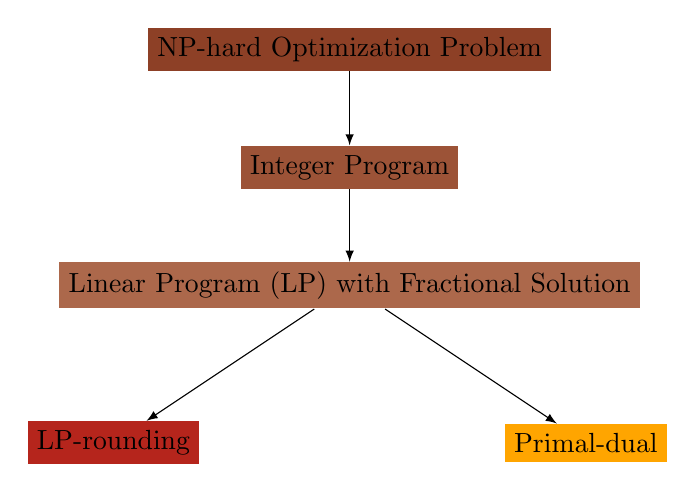
\begin{tikzpicture}
    \node[fill=Sepia!70] (npo) at (0,0) {NP-hard Optimization Problem};
    \node[fill=Sepia!60] (ip) at (0,-1.5) {Integer Program};
    \node[fill=Sepia!50] (lp) at (0,-3) {Linear Program (LP) with Fractional Solution};
    \node[fill=BrickRed]  (rounding) at (-3,-5) {LP-rounding};
    \node[fill=Orange] (primal) at (3,-5) {Primal-dual};

    \draw[->,>=latex] (npo) -- (ip);
    \draw[->,>=latex] (ip) -- (lp);
    \draw[->,>=latex] (lp) -- (rounding);
    \draw[->,>=latex] (lp) -- (primal);
  \end{tikzpicture}
  \end{center}
  
\end{frame}

%%%%%%%%%%%%%%%%%%%%%%%%%%%%%%%%%%%%%%%%%%%%%%%%%%%
%% Results Highlight
%%%%%%%%%%%%%%%%%%%%%%%%%%%%%%%%%%%%%%%%%%%%%%%%%%%
\begin{frame}
  \frametitle{Results Highlight}
  \large{
  \begin{itemize}
    \addtolength{\itemsep}{1\baselineskip}
  \item \color{blue}LP-rounding: 1.575-approximation
  \item \color{blue}LP-rounding: asymptotic ratio of 1 when all demands large
  \item \color{blue}Primal-dual: $H_n$-approximation
  \item \color{blue}Primal-dual: Example of $\Omega(\log n / \log\log n)$ for dual-fitting
  \end{itemize}}
\end{frame}

%%%%%%%%%%%%%%%%%%%%%%%%%%%%%%%%%%%%%%%%%%%%%%%%%%%%
%% Compare three problems
%%%%%%%%%%%%%%%%%%%%%%%%%%%%%%%%%%%%%%%%%%%%%%%%%%%% 
\begin{frame}
  \frametitle{Relation between Problems}
  \begin{center}
  \begin{tabular}{l  l  l}
    \rowcolor{light-gray}
    \textcolor{blue}{FTFP} & $r_j \geq 1$ & $< \infty$ facility per site\\
    \rowcolor{light-gray}
    UFL  & $r_j = 1$ & $\leq 1$ facility per site\\
    \rowcolor{light-gray}
    FTFL & $r_j \geq 1$ & $\leq 1$ facility per site\\
  \end{tabular}
  \end{center}
  
  \vspace{.3in}
  \pause
  \hfsetbordercolor{red!50}
  \hfsetfillcolor{blue!10}
  \large{
  \begin{equation*}
    \tikzmarkin{a}(0.3,-0.6)(-0.3,0.75)
    \text{UFL} \preceq \text{\textcolor{blue}{FTFP}} \preceq \text{FTFL}
    \tikzmarkend{a}
  \end{equation*}
  }

  \pause
  \begin{minipage}{.45\linewidth}
  \vspace{.3in}
  \begin{center}
    \begin{tabular}{l l}
      \rowcolor{Yellow}
      \multicolumn{2}{c}{LP-rounding}\\
      \hline
      \rowcolor{GreenYellow}
      UFL & \\
      \rowcolor{GreenYellow}
      \textcolor{blue}{FTFP} & \multirow{-2}{*}{1.575}\\
      \rowcolor{Cyan}
      FTFL & 1.7245\\
    \end{tabular}
    \end{center}
  \end{minipage}
  \pause
  \begin{minipage}{.45\linewidth}
  \vspace{.3in}
  \begin{center}
    \begin{tabular}{l l}
      \rowcolor{Yellow}
      \multicolumn{2}{c}{Primal-dual}\\
      \hline
      \rowcolor{GreenYellow}
      UFL & 1.52\\
      \rowcolor{Cyan}
      \textcolor{blue}{FTFP} & \\
      \rowcolor{Cyan}
      FTFL & \multirow{-2}{*}{$O(\log n)$}\\
    \end{tabular}
    \end{center}
  \end{minipage}
\end{frame}

\section[Related Work]{Related Work}

\subsection{UFL}
%%%%%%%%%%%%%%%%%%%%%%%%%%%%%%%%%%%%%%%%%%%%%%%
%% UFL and its results
%%%%%%%%%%%%%%%%%%%%%%%%%%%%%%%%%%%%%%%%%%%%%%%
%%% UFL example
%%\begin{frame}
%%  \frametitle{Uncapacitated Facility Location Problem (UFL)}
%%  \begin{block}{}
%%    All demands are 1, each site can open only one facility    
%%  \end{block}
%%
%%  \begin{columns}
%%    \column{0.5\textwidth}
%%    \begin{figure}[ht]
%%      \centering
%%      \begin{tikzpicture}[scale=0.4]
%%        \node[fill=blue!50,minimum size=.2cm] (fac3) at (0,2) {$3$};
%%        \node[fill=blue!50,minimum size=.2cm] (fac2) at (0,5) {$2$};
%%        \node[fill=blue!50,minimum size=.2cm] (fac1) at (0,8) {$1$};
%%
%%        \node[circle,fill=green!50,minimum size=.2cm] (client4) at (6,0) {$4$};
%%        \node[circle,fill=green!50,minimum size=.2cm] (client3) at (6,3) {$3$};
%%        \node[circle,fill=green!50,minimum size=.2cm] (client2) at (6,6) {$2$};
%%        \node[circle,fill=green!50,minimum size=.2cm] (client1) at (6,9) {$1$};
%%
%%        \node[right] (demand1) at (6,-1) {$r_4=1$};
%%        \node[right] (demand2) at (6,2) {$r_3=1$};
%%        \node[right] (demand3) at (6,5) {$r_2=1$};
%%        \node[right] (demand4) at (6,8) {$r_1=1$};
%%    
%%        \node (label1) at (3,-3) {Instance};
%%      \end{tikzpicture}      
%%    \end{figure}
%%    % solution
%%    \column<2->{0.5\textwidth}
%%    \begin{figure}[ht]
%%      \centering
%%      \begin{tikzpicture}[scale=0.4]
%%        \node[fill=blue!75,minimum size=.2cm] (fac3) at (0,2) {$3$};
%%        \node[fill=blue!75,minimum size=.2cm] (fac2) at (0,5) {$2$};
%%        \node[fill=blue!25,minimum size=.2cm] (fac1) at (0,8) {$1$};
%%
%%        \node[circle,fill=green!50,minimum size=.2cm] (client4) at (6,0) {$4$};
%%        \node[circle,fill=green!50,minimum size=.2cm] (client3) at (6,3) {$3$};
%%        \node[circle,fill=green!50,minimum size=.2cm] (client2) at (6,6) {$2$};
%%        \node[circle,fill=green!50,minimum size=.2cm] (client1) at (6,9) {$1$};
%%
%%        \foreach \from/\to in {fac2/client1,fac2/client4,fac3/client2,fac3/client3}
%%        \draw (\from)--(\to);
%%
%%        \node (label2) at (3,-3) {Solution};
%%      \end{tikzpicture}
%%    \end{figure}
%%  \end{columns}
%%\end{frame}

\begin{frame}
  \frametitle{Related Work for UFL}

  \centering
  {\Large
    \textcolor{blue}
    {Approximation Results for UFL}
  }

  \vspace{.1in}
  \centering
  \begin{tabular}{ l l l l }
    \rowcolor{GreenYellow}
    Shmoys, Tardos and Aardal & 1997 & 3.16 & LP-rounding\\
    \rowcolor{GreenYellow}
    Chudak & 1998 & 1.736 & LP-rounding\\
    \rowcolor{GreenYellow}
    Sviridenko & 2002 & 1.58 & LP-rounding\\

    \rowcolor{Pink}
    Jain and Vazirani & 2001 & 3 & primal-dual\\
    \rowcolor{ProcessBlue}
    Jain {\etal} & 2002 & 1.61 & greedy\\
    \rowcolor{ProcessBlue}
    Mahdian {\etal} & 2002 & 1.52 & greedy\\
	\rowcolor{LightGreen}
    Arya {\etal} & 2004 & 3 & local search\\
    \rowcolor{SkyBlue}
    Byrka & 2007 & 1.5 & hybrid\\
    \rowcolor{SkyBlue}
    Li & 2011 & 1.488 & hybrid \\
	& & &\\
	\textcolor{blue}{Lower Bound}
	& & & \\
    & & & \\
    \rowcolor{Yellow}
    Guha and Khuller & 1998 & 1.463 &\\
  \end{tabular}
\end{frame}

\subsection{FTFL}
%%%%%%%%%%%%%%%%%%%%%%%%%%%%%%%%%%%%%%%%%%%%%%%
%% FTFL and its results
%%%%%%%%%%%%%%%%%%%%%%%%%%%%%%%%%%%%%%%%%%%%%%%
%%% FTFL example
%%\begin{frame}
%%  \frametitle{Fault-Tolerant Facility Location Problem (FTFL)}
%%  \begin{block}{}
%%    Demands may be more than 1, each site can open only one
%%    facility
%%  \end{block}
%%
%%  \begin{columns}
%%    \column{0.5\textwidth}
%%    \begin{figure}[ht]
%%      \centering
%%      \begin{tikzpicture}[scale=0.4]
%%        \node[fill=blue!50,minimum size=.2cm] (fac3) at (0,2) {$3$};
%%        \node[fill=blue!50,minimum size=.2cm] (fac2) at (0,5) {$2$};
%%        \node[fill=blue!50,minimum size=.2cm] (fac1) at (0,8) {$1$};
%%
%%        \node[circle,fill=green!50,minimum size=.2cm] (client1) at (6,0) {$4$};
%%        \node[circle,fill=green!50,minimum size=.2cm] (client2) at (6,3) {$3$};
%%        \node[circle,fill=green!50,minimum size=.2cm] (client3) at (6,6) {$2$};
%%        \node[circle,fill=green!50,minimum size=.2cm] (client4) at (6,9) {$1$};
%%
%%        \node[right] (demand1) at (6,-1) {$r_4=2$};
%%        \node[right] (demand2) at (6,2) {$r_3=1$};
%%        \node[right] (demand3) at (6,5) {$r_2=1$};
%%        \node[right] (demand4) at (6,8) {$r_1=2$};
%%
%%        \node (label1) at (3,-3) {Instance};    
%%      \end{tikzpicture}      
%%    \end{figure}
%%    \column<2->{0.5\textwidth}
%%    \begin{figure}[ht]
%%      \begin{center}
%%      \begin{tikzpicture}[scale=0.4]
%%        \node[fill=blue!75,minimum size=.2cm] (fac3) at (0,2) {$3$};
%%        \node[fill=blue!75,minimum size=.2cm] (fac2) at (0,5) {$2$};
%%        \node[fill=blue!75,minimum size=.2cm] (fac1) at (0,8) {$1$};
%%
%%        \node[circle,fill=green!50,minimum size=.2cm] (client4) at (6,0) {$4$};
%%        \node[circle,fill=green!50,minimum size=.2cm] (client3) at (6,3) {$3$};
%%        \node[circle,fill=green!50,minimum size=.2cm] (client2) at (6,6) {$2$};
%%        \node[circle,fill=green!50,minimum size=.2cm] (client1) at (6,9) {$1$};
%%    
%%        \foreach \from/\to in {fac1/client1,fac1/client2,fac1/client3,fac2/client1,fac2/client4,fac3/client4}
%%        \draw (\from)--(\to);
%%
%%        \node (label2) at (3,-3) {Solution};
%%      \end{tikzpicture}
%%      \end{center}
%%    \end{figure}
%%  \end{columns}
%%\end{frame}

\begin{frame}
  \frametitle{Related Work for FTFL}
  
  \centering
  {\Large
    \textcolor{blue}
    {Approximation Algorithms for FTFL}
  }

    \vspace{.3in}
    \centering
    \begin{tabular}{ l l l l }
      \rowcolor{GreenYellow}
      Jain and Vazirani & 2000 & $3\ln \max_j r_j$ & primal-dual\\
      \rowcolor{SkyBlue}
      Guha {\etal} & 2001 & 4 & LP-rounding\\
      \rowcolor{SkyBlue}
      Swamy, Shmoys & 2008 & 2.076 & LP-rounding\\
      \rowcolor{SkyBlue}
      Byrka {\etal} & 2010 & 1.7245 & LP-rounding\\
    \end{tabular}
    \vspace{.5in}

    \begin{block}{} 
      No primal-dual algorithms for FTFL with constant
      ratio.
    \end{block}
    
\end{frame}

%%%%%%%%%%%%%%%%%%%%%%%%%%%%%%%%%%%%%%%%%%%%%%%%%%%%%%%
%%%%%%%%%%%%%%%% FTFP results %%%%%%%%%%%%%%%%%%%%%%%%%%
%%%%%%%%%%%%%%%%%%%%%%%%%%%%%%%%%%%%%%%%%%%%%%%%%%%%%%%
\begin{frame}
  \frametitle{Work on FTFP (Dissertation Topic)}
  
  {\Large
    \textcolor{blue}
    {Approximation Algorithms for FTFP}
  }

    \vspace{.3in}
    \begin{tabular}{ l l l l }
	  \rowcolor{GreenYellow}
      Xu and Shen & 2009 &  & Introduced FTFP\\
      \rowcolor{Pink}
      Liao and Shen & 2011 & 1.861 & Dual-fitting (for special case)\\
      \rowcolor{SkyBlue}
      Yan and Chrobak & 2011 & 3.16 & LP-rounding\\
      \rowcolor{SkyBlue}
      Yan and Chrobak & 2012 & 1.575 & LP-rounding\\
      \rowcolor{Purple!20}
      Yan and Chrobak & \multicolumn{2}{l}{preliminary results} & Dual-fitting (for general case)\\
    \end{tabular}

\end{frame}


%% 2. Results: 1.575 rounding, hard example on dual-fitting

%% 3. Techniques:
%% 3.1 Demand Reduction: why, what (end product) and how (take floor)
%%     implication: reduction to FTFL, 1 + O(m/Q) approximation
%% 3.2 Adaptive Partitioning: why, what and how
%%     why: to use UFL-like rounding
%%     what: facility points and unit demand points, \barx and \bary with mu and nu
%%           properties...
%%     how: unit chunk, best client, primary, non-primary, overlap of neighborhood
%%%%%%%%%%%%%%%%%%%%%%%%%%%%%%%%%%%%%%%%%%%%%%%%%%%%%%%%%%%%%%%%%%%%%%%%%%%%%%%%%%%%%%%%%%%%%%%%%%%%
%%% LP-Formulation
%%%%%%%%%%%%%%%%%%%%%%%%%%%%%%%%%%%%%%%%%%%%%%%%%%%%%%%%%%%%%%%%%%%%%%%%%%%%%%%%%%%%%%%%%%%%%%%%%%%%
\section[Techniques]{Techniques}

%%%%%%%%%%%%%%%%%%%%%%%%%%%%%%%%%%%%%%%%%%%%%%%%%%%%%%%%%%%%%%%%%%%%%%%%%%%%%%%%%%%%%%%%%%%%%%%%%%%%
%%% Techniques
%%%%%%%%%%%%%%%%%%%%%%%%%%%%%%%%%%%%%%%%%%%%%%%%%%%%%%%%%%%%%%%%%%%%%%%%%%%%%%%%%%%%%%%%%%%%%%%%%%%%
\begin{frame}
  \frametitle{Techniques}

  \begin{itemize}\addtolength{\itemsep}{2\baselineskip}

  \item {\Large \textcolor{blue}{Demand Reduction}}
    \vspace{.1in}
    \begin{itemize}\addtolength{\itemsep}{1\baselineskip}
    \item {\large Reduce all $r_j$ to polynomial values (to ensure polynomial time of
						rounding)}
    \item {\large $\rho$-approx for reduced instance $\Rightarrow$ $\rho$-approx for original instance }
    \end{itemize}
    
  \item {\Large \textcolor{blue}{Adaptive Partitioning}}
    \vspace{.1in}
    \begin{itemize}\addtolength{\itemsep}{1\baselineskip}
    \item {\large Split sites into facilities and clients into unit demands}
    \item {\large Split associated fractional values}
    \item {\large Properties ensure rounding similar to UFL can be applied}
    \end{itemize}
  \end{itemize}
\end{frame}

\begin{frame}
  \frametitle{LP Formulation for FTFP}
  \begin{itemize}
  \item \textcolor{red}{$y_i$} = number of facilities open at site $i\in \sitesset$
  \item \textcolor{red}{$x_{ij}$} = number of connections from client $j\in
    \clientset$ to site $i \in \sitesset$
  \end{itemize}
  %%%%%%%%%%% 
  \begin{alignat*}{3}
    \text{(Primal)} \quad\textrm{minimize}\quad \sum f_iy_i &+ \sum d_{ij}x_{ij}&
    \\ \notag
    \textrm{subject to}\quad y_i - x_{ij} &\geq 0  & &\forall i,j
    \\ \notag
    \sum x_{ij} &\geq r_j & &\forall j
    \\ \notag
    x_{ij} \geq 0, y_i &\geq 0 & &\forall i,j
  \end{alignat*}
  %%%%%%%%%%%%
  \begin{alignat*}{3}
  \text{(Dual)}\quad  \textrm{maximize}\quad \sum r_j\, \alpha_j&
    \\ \notag
    \textrm{subject to} \quad 
      \sum \beta_{ij} &\leq f_i  &\quad\quad			&\forall i
    \\ \notag
    \alpha_{j} - \beta_{ij} 	&\leq  d_{ij}       &                 & \forall i,j
    \\ \notag
    \alpha_j \geq 0, \beta_{ij} &\geq 0           &            & \forall i,j
  \end{alignat*}
  %%%%%%%%%%%
\end{frame}

%%%%%%%%%%%%%%%%%%%%%%%%%%%%%%%%%%%%%%%%%%%%%%%%%%%%%%%%%%%%%%%%%%%%%%%%%%%%%%%%%%%%%%%%%%%%%%%%%%%%
%%% Algorithm for FTFP - Demand Reduction
%%%%%%%%%%%%%%%%%%%%%%%%%%%%%%%%%%%%%%%%%%%%%%%%%%%%%%%%%%%%%%%%%%%%%%%%%%%%%%%%%%%%%%%%%%%%%%%%%%%%
\subsection[Demand Reduction]{Demand Reduction}
\begin{frame}
  \frametitle{Algorithm for FTFP}
  \begin{center}
  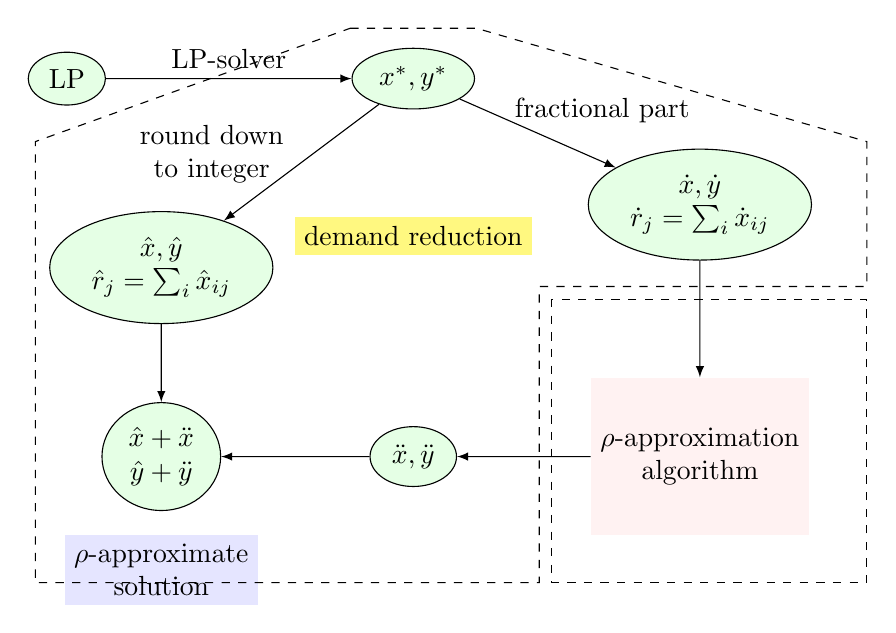
\begin{tikzpicture}[auto,scale=.8,every text node part/.style={align=center}]
    \node[draw,ellipse,fill=green!10] (lpform) at (-5.5,9) {LP};
    \node[draw,ellipse,fill=green!10] (lpsoln) at (0,9) {$x^\ast, y^\ast$};
    \node[draw,ellipse,fill=green!10] (intpart) at (-4,6) {$\hatx, \haty$ \\ $\hatr_j = \sum_i \hatx_{ij}$};
    \node[draw,ellipse,fill=green!10] (fracpart) at (4.55,7) {$\dotx, \doty$ \\ $\dotr_j = \sum_i \dotx_{ij}$};
    \node[fill=red!5,minimum size=2cm] (part) at (4.55,3) {$\rho$-approximation\\ algorithm};
    \node[draw,ellipse,fill=green!10] (fracsoln) at (0,3) {$\ddot x, \ddot y$};

    \node[draw, ellipse,fill=green!10] (soln) at (-4,3) {$\hatx + \ddot x$ \\ $\haty + \ddot y$};

    \node[fill=blue!10] (solnlabel) at (-4,1.2) {$\rho$-approximate \\ solution};

    \draw[->,>=latex] (lpform) to node {LP-solver} (lpsoln);
    \draw[->,>=latex] (lpsoln) to (intpart);
    \node (label1) at (-3.2,7.8) {round down \\ to integer};
    \draw[->,>=latex] (lpsoln) to (fracpart);
    \node (label2) at (3,8.5) {fractional part};
    \draw[->,>=latex] (fracpart) to node(edge1){} (part);
    \draw[->,>=latex] (part) to node (edge2){} (fracsoln);
    \draw[->,>=latex] (intpart) to (soln);
    \draw[->,>=latex] (fracsoln) to (soln);

    \draw[dashed] (-1,9.8) -- (1,9.8) -- (7.2,8) -- (7.2,5.7) -- (2,5.7)
    -- (2,1) -- (-6,1) -- (-6,8) -- (-1,9.8);

	\draw[dashed] (2.2,5.5) -- (2.2,1) -- (7.2,1) -- (7.2,5.5) -- (2.2,5.5);

    \node[fill=yellow!50] at (0,6.5) {demand reduction};
  \end{tikzpicture}
  \end{center}
\end{frame}

%%%%%%%%%%%%%%%%%%%%%%%%%%%%%%%%%%%%%%%%%%%%%%%%%%%%%%%%%%%%%%%%%%%%%%%%%%%%%%%%%%%%%%%%%%%%%%%%%%%%
%%% Algorithm for FTFP
%%%%%%%%%%%%%%%%%%%%%%%%%%%%%%%%%%%%%%%%%%%%%%%%%%%%%%%%%%%%%%%%%%%%%%%%%%%%%%%%%%%%%%%%%%%%%%%%%%%%

\begin{frame}
  \frametitle{Algorithm for FTFP}
  \begin{center}
  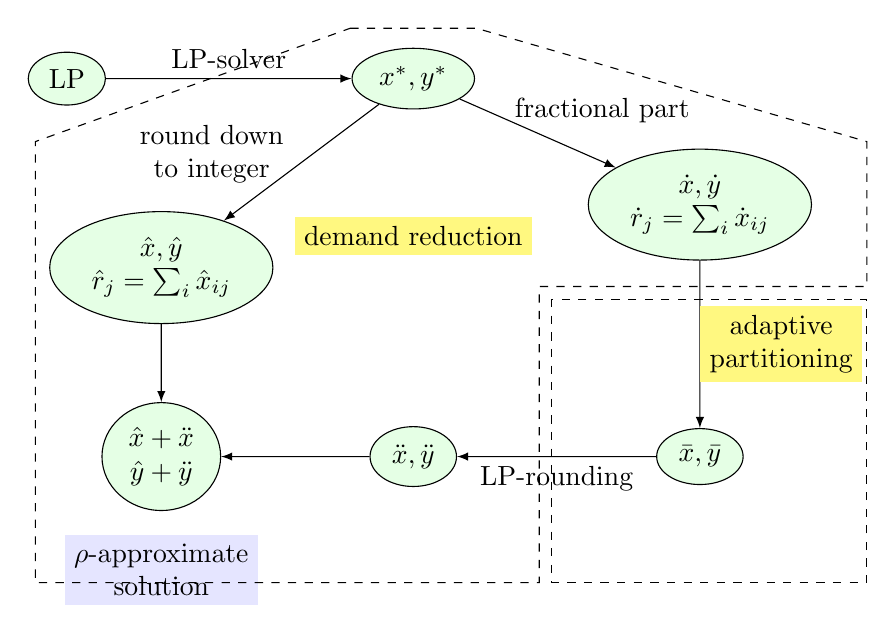
\begin{tikzpicture}[auto,scale=.8,every text node part/.style={align=center}]
    \node[draw,ellipse,fill=green!10] (lpform) at (-5.5,9) {LP};
    \node[draw,ellipse,fill=green!10] (lpsoln) at (0,9) {$x^\ast, y^\ast$};
    \node[draw,ellipse,fill=green!10] (intpart) at (-4,6) {$\hatx, \haty$ \\ $\hatr_j = \sum_i \hatx_{ij}$};
    \node[draw,ellipse,fill=green!10] (fracpart) at (4.55,7) {$\dotx, \doty$ \\ $\dotr_j = \sum_i \dotx_{ij}$};
    \node[draw,ellipse,fill=green!10] (part) at (4.55,3) {$\barx,\bary$};
    \node[draw,ellipse,fill=green!10] (fracsoln) at (0,3) {$\ddot x, \ddot y$};

    \node[draw, ellipse,fill=green!10] (soln) at (-4,3) {$\hatx + \ddot x$ \\ $\haty + \ddot y$};

    \node[fill=blue!10] (solnlabel) at (-4,1.2) {$\rho$-approximate \\ solution};

    \draw[->,>=latex] (lpform) to node {LP-solver} (lpsoln);
    \draw[->,>=latex] (lpsoln) to (intpart);
    \node (label1) at (-3.2,7.8) {round down \\ to integer};
    \draw[->,>=latex] (lpsoln) to (fracpart);
    \node (label2) at (3,8.5) {fractional part};
    \draw[->,>=latex] (fracpart) to node[fill=yellow!50] (edge1) { adaptive \\ partitioning} (part);
    \draw[->,>=latex] (part) to node (edge2) {LP-rounding} (fracsoln);
    \draw[->,>=latex] (intpart) to (soln);
    \draw[->,>=latex] (fracsoln) to (soln);

    \draw[dashed] (-1,9.8) -- (1,9.8) -- (7.2,8) -- (7.2,5.7) -- (2,5.7)
    -- (2,1) -- (-6,1) -- (-6,8) -- (-1,9.8);

	\draw[dashed] (2.2,5.5) -- (2.2,1) -- (7.2,1) -- (7.2,5.5) -- (2.2,5.5);

    \node[fill=yellow!50] at (0,6.5) {demand reduction};
  \end{tikzpicture}
  \end{center}
\end{frame}

%%%%%%%%%%%%%%%%%%%%%%%%%%%%%%%%%%%%%%%%%%%%%
%%% demand reduction
%%%%%%%%%%%%%%%%%%%%%%%%%%%%%%%%%%%%%%%%%%%%%
\begin{frame}
  \setbeamercovered{transparent=50}
  \frametitle{Techniques}
  \begin{itemize}\addtolength{\itemsep}{1\baselineskip}

  \item<1> {\Large \textcolor{blue}{Demand Reduction}}
    \vspace{.1in}
    \begin{itemize}\addtolength{\itemsep}{1\baselineskip}
    \item  {\large Reduce all $r_j$ to polynomial values (to ensure polynomial time of
						rounding)}
    \item  {\large $\rho$-approx for reduced instance $\Rightarrow$ $\rho$-approx for original instance }
    \end{itemize}
    
  \item<0> {\Large {Adaptive Partitioning}}
    \vspace{.1in}
    \begin{itemize}\addtolength{\itemsep}{1\baselineskip}
    \item {\large Split sites into facilities and clients into unit demands}
    \item {\large Split associated fractional values}
    \item {\large Properties ensure rounding similar to UFL can be applied}
    \end{itemize}
  \end{itemize}
\end{frame}

\begin{frame}
  \frametitle{Demand Reduction}

  \large{\textcolor{blue}{Implementation}}

  \begin{itemize}
  \item Solving LP for $(\bfx^\ast, \bfy^\ast)$.
  \item $(\hat\bfx, \hat\bfy) = (\bfx^\ast, \bfy^\ast)$ round down to integer
  \item $(\dot\bfx, \dot\bfy) = (\bfx^\ast, \bfy^\ast) - (\hat\bfx, \hat\bfy)$, fractional part
  \item $\hat r_j = \sum_{i}\hat x_{ij}$ for $\hat\calI$, $\dot r_j = r_j - \hat r_j$ for $\dot\calI$
  \item $(\hat\bfx, \hat\bfy)$ (integral) feasible and optimal for $\hat\calI$
  \item $(\dot\bfx, \dot\bfy)$ (fractional) feasible and optimal for $\dot\calI$
  \end{itemize}
  
  \large{\textcolor{blue}{Properties}}

  \begin{itemize}
  \item $\dotr_j = \poly(|\sitesset|)$
  \item $\rho$-approx for $\dot \calI$ implies $\rho$-approx for $\calI$
  \end{itemize}
\end{frame}

\begin{frame}
  \frametitle{Demand Reduction: Consequences}
  \begin{block}{}
    FTFP to FTFL, 1.7245-approximation    
  \end{block}
  \begin{itemize}
  \item Sites into facilities
  \item Clients with demand $r_j$
  \item FTFL size polynomial because demand reduction
  \end{itemize}

  \begin{block}{}
    Ratio $1 + O(|F| / Q)$ for $Q = \min_j r_j$,
    approaches $1$ when $Q$ is large
  \end{block}
  \begin{itemize}
  \item Next slide
  \end{itemize}
\end{frame}

\begin{frame}
  \frametitle{Ratio $1+O(|F|/Q)$ for FTFP}
  \begin{center}
  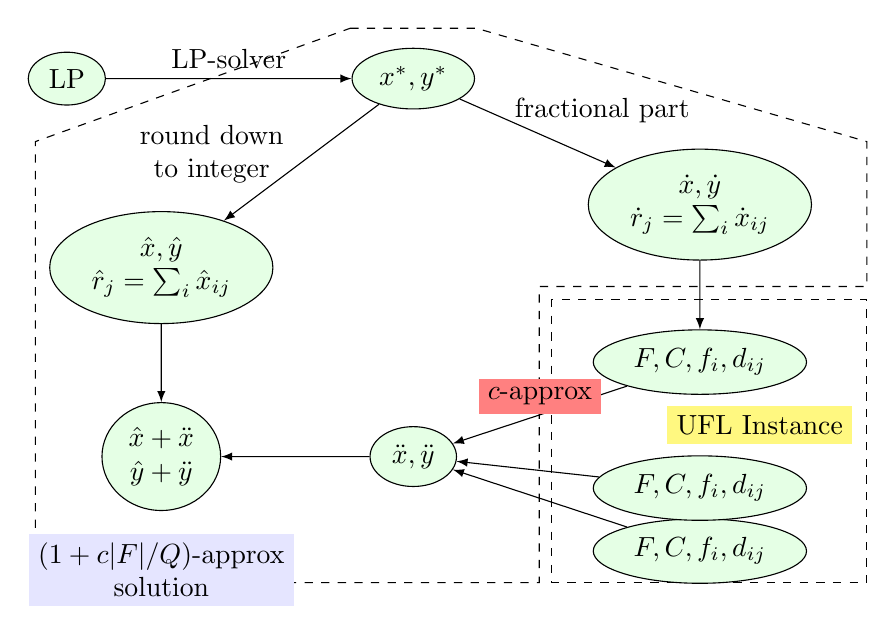
\begin{tikzpicture}[auto,scale=.8,every text node part/.style={align=center}]
    \node[draw,ellipse,fill=green!10] (lpform) at (-5.5,9) {LP};
    \node[draw,ellipse,fill=green!10] (lpsoln) at (0,9) {$x^\ast, y^\ast$};
    \node[draw,ellipse,fill=green!10] (intpart) at (-4,6) {$\hatx, \haty$ \\ $\hatr_j = \sum_i \hatx_{ij}$};
    \node[draw,ellipse,fill=green!10] (fracpart) at (4.55,7) {$\dotx, \doty$ \\ $\dotr_j = \sum_i \dotx_{ij}$};


    \node[draw,ellipse,fill=green!10] (fracsoln) at (0,3) {$\ddot x, \ddot y$};

    \node[draw, ellipse,fill=green!10] (soln) at (-4,3) {$\hatx + \ddot x$ \\ $\haty + \ddot y$};

    \draw[->,>=latex] (lpform) to node {LP-solver} (lpsoln);
    \draw[->,>=latex] (lpsoln) to (intpart);
    \node (label1) at (-3.2,7.8) {round down \\ to integer};
    \draw[->,>=latex] (lpsoln) to (fracpart);

    \node (label2) at (3,8.5) {fractional part};
    \draw[->,>=latex] (intpart) to (soln);
    \draw[->,>=latex] (fracsoln) to (soln);

    \draw[dashed] (-1,9.8) -- (1,9.8) -- (7.2,8) -- (7.2,5.7) -- (2,5.7)
    -- (2,1) -- (-6,1) -- (-6,8) -- (-1,9.8);

    \draw[dashed] (2.2,5.5) -- (2.2,1) -- (7.2,1) -- (7.2,5.5) -- (2.2,5.5);

    \pause
    \node[draw,ellipse,fill=green!10] (part1) at (4.55,1.5) {$F,C,f_i,d_{ij}$};
    \node[draw,ellipse,fill=green!10] (part2) at (4.55,2.5) {$F,C,f_i,d_{ij}$};
    \node[draw,ellipse,fill=green!10] (part3) at (4.55,4.5) {$F,C,f_i,d_{ij}$};
    \node[fill=yellow!50] (UFL) at (5.5,3.5) {UFL Instance};

    \draw[->,>=latex] (part1) to (fracsoln);
    \draw[->,>=latex] (part2) to (fracsoln);
    \draw[->,>=latex] (part3) to node (alg)[above,fill=red!50] {$c$-approx} (fracsoln);

    \draw[->,>=latex] (fracpart) to (part3);

    \node[fill=blue!10] (solnlabel) at (-4,1.2) {$(1+c|F|/Q)$-approx\\ solution};
  \end{tikzpicture}
  \end{center}
\end{frame}


%%%%%%%%%%%%%%%%%%%%%%%%%%%%%%%%%%%%%%%%%%%%%%%%%%%%%%%%%%%%%%%%%%%%%%%%%%%%%%%%%%%%%%%%%%%%%%%%%%%%
%%% Adaptive Partitioning, site -> client
%%%%%%%%%%%%%%%%%%%%%%%%%%%%%%%%%%%%%%%%%%%%%%%%%%%%%%%%%%%%%%%%%%%%%%%%%%%%%%%%%%%%%%%%%%%%%%%%%%%%
\subsection[Adaptive Partitioning]{Adaptive Partitioning}
\begin{frame}
  \setbeamercovered{transparent=50}
  \frametitle{Techniques}
  \begin{itemize}\addtolength{\itemsep}{1\baselineskip}

  \item<0> {\Large {Demand Reduction}}
    \vspace{.1in}
    \begin{itemize}\addtolength{\itemsep}{1\baselineskip}
    \item  {\large Reduce all $r_j$ to polynomial values (to ensure polynomial time of
						rounding)}
    \item  {\large $\rho$-approx for reduced instance $\Rightarrow$ $\rho$-approx for original instance }
    \end{itemize}
    
  \item<1> {\Large \textcolor{blue}{Adaptive Partitioning}}
    \vspace{.1in}
    \begin{itemize}\addtolength{\itemsep}{1\baselineskip}
    \item {\large Split sites into facilities and clients into unit demands}
    \item {\large Split associated fractional values}
    \item {\large Properties ensure rounding similar to UFL can be applied}
    \end{itemize}
  \end{itemize}
\end{frame}

%%%%%%%%%%%%%%%%%%%%%%%%%%%%%%%%%%%%%%%%%%%%%%%%%%%%%%%%%%%%%%%%%%%%%%%%%%%%%%%%%%%%%%%%%%%%%%%%%%%%
%%% Adaptive Partitioning, partition site into facilities, client into demands
%%%%%%%%%%%%%%%%%%%%%%%%%%%%%%%%%%%%%%%%%%%%%%%%%%%%%%%%%%%%%%%%%%%%%%%%%%%%%%%%%%%%%%%%%%%%%%%%%%%%

\begin{frame}
  \frametitle{Adaptive Partitioning}
  \setbeamercovered{invisible}

  \begin{center}
  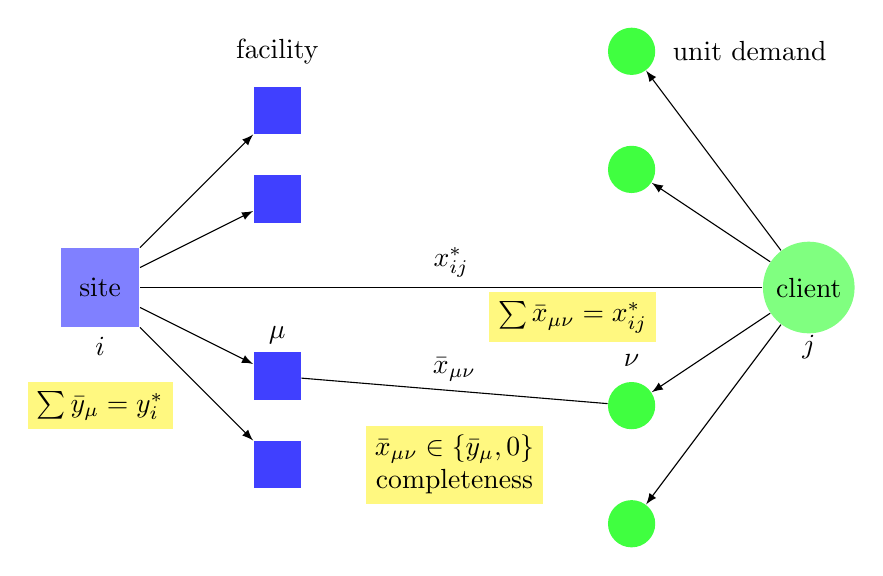
\begin{tikzpicture}[scale=.75,every text node part/.style={align=center}]
    % site to facility
    \node[fill=blue!50,minimum size=1cm] (site) at (0,0) {site};
    \node (siteilabel) at (0,-1) {$i$};
    \node[circle, fill=green!50,minimum size=1cm] (client) at (12,0) {client};
    \node (jlabel) at (12,-1) {$j$};

    \draw[above] (site) to node (dummy) {$x_{ij}^\ast$} (client);

    \pause
    \node[fill=blue!75,minimum size=.6cm] (fac1) at (3,3) {};
    \node[fill=blue!75,minimum size=.6cm] (fac2) at (3,1.5) {};
    \node[fill=blue!75,minimum size=.6cm] (fac3) at (3,-1.5) {};
    \node[fill=blue!75,minimum size=.6cm] (fack) at (3,-3) {};

    \foreach \from in {site}
    \foreach \to in {fac1,fac2,fac3,fack}
    \draw[->,>=latex] (\from) -- (\to);

    \node (faclabel) at (3,4) {facility};
    \node[below] (faclabel) at (3,-.5) {$\mu$};

    \node[fill=yellow!50] (sumyi) at (0,-2) {$\sum \bary_{\mu} = y_i^\ast$};

    \pause
    % client to demand
    \node[circle, fill=green!75, minimum size=.6cm] (demand1) at (9,4) {};
    \node[circle, fill=green!75, minimum size=.6cm] (demand2) at (9,2) {};

    \node[circle, fill=green!75, minimum size=.6cm] (demand3) at (9,-2) {};
    \node[circle, fill=green!75, minimum size=.6cm] (demandk) at (9,-4) {};
    \foreach \from in {client}
    \foreach \to in {demand1, demand2, demand3, demandk}
    \draw[->,>=latex] (\from) -- (\to);

    \node (demandlabel) at (11,4) {unit demand};
    \node[above] (nulabel) at (9,-1.5) {$\nu$};

    \pause
	\draw[above] (fac3) to node (xval) {$\barx_{\mu\nu}$} (demand3);
    \node[fill=yellow!50] (comp) at (6,-3) {$\barx_{\mu\nu} \in \{\bary_{\mu}, 0\}$ \\ completeness};
    \node[fill=yellow!50] (sumxij) at (8,-.5) {$\sum \barx_{\mu\nu} = x_{ij}^\ast$};
    % xval

  \end{tikzpicture}
  \begin{block}<4>{} Now round each $\bary_{\mu}$ and $\barx_{\mu\nu}$ to 0 or 1...
    \end{block}

  \end{center}
\end{frame}

%%%%%%%%%%%%%%%%%%%%%%%%%%%%%%%%%%%%%%%%%%%%%%%%%%%%%%%%%%%%%%%%%%%%%%%%%%%%%%%%%%%%%%%%%%%%%%%%%%%%
%%% Neigbhorhood
%%%%%%%%%%%%%%%%%%%%%%%%%%%%%%%%%%%%%%%%%%%%%%%%%%%%%%%%%%%%%%%%%%%%%%%%%%%%%%%%%%%%%%%%%%%%%%%%%%%%

\begin{frame}
  \frametitle{Neighborhood of Demand}

  \begin{center}
  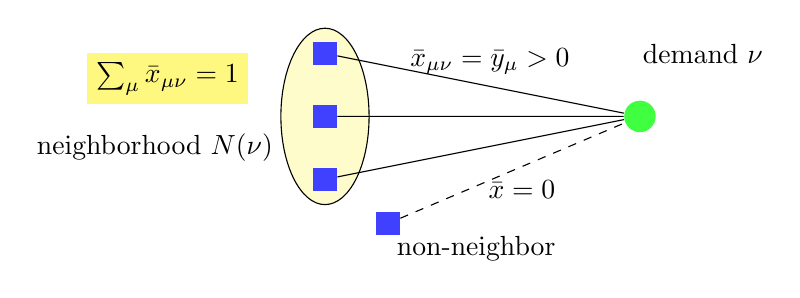
\begin{tikzpicture}[scale = 0.8,auto,every text node part/.style={align=left}]
  
  \draw[fill=yellow!20] (3,4) ellipse (0.7cm and 1.4cm);
    \node[fill=blue!75,minimum size=.3cm] (fac1) at (3,5) {};
    \node[fill=blue!75,minimum size=.3cm] (fac2) at (3,4) {};
    \node[fill=blue!75,minimum size=.3cm] (fac3) at (3,3) {};
    \node[fill=blue!75,minimum size=.3cm] (fac4) at (4,2.3) {};

    \node[circle,fill=green!75,minimum size=.4cm] (demand) at (8,4){};

    \draw[solid] (fac1) to node[above] {\ \ $\barx_{\mu\nu} = \bary_{\mu} > 0$} (demand);
	\draw[solid] (fac2) to (demand);
	\draw[solid] (fac3) to (demand);

    \draw[dashed] (fac4) to node[below] (zerolabel) {\ \ $\barx = 0$} (demand);

    \node (faclabel) at (0.3,3.5) {neighborhood $N(\nu)$};
    \node (otherlabel) at (5.4,1.9) {non-neighbor};
    \node (demandlabel) at (9,5) {demand $\nu$};
    
    \node[fill=yellow!50] (sumlabel) at (0.5,4.6) {$\sum_\mu \barx_{\mu\nu} = 1$};
  \end{tikzpicture}
	\end{center}

        \vspace{-.3in}
        \setbeamercolor{postit}{fg=blue,bg=yellow}
        \begin{beamercolorbox}[sep=.5em,wd=4cm]{postit}
          $\nu$ needs $1$ facility...
        \end{beamercolorbox}

\pause
\noindent
\begin{minipage}{2in}	
\textcolor{Brown}{Strategy 1:} for each $\nu$, open one $\mu\in N(\nu)$ with prob. $\bary_\mu$ 
		\begin{itemize}
			\item optimal connection cost
			\item large facility cost 
		\end{itemize}
\end{minipage}
\ \ 
\begin{minipage}{2in}
\textcolor{Brown}{Strategy 2:} do this for demands with disjoint neighborhoods
		\begin{itemize}
			\item optimal facility cost
			\item large connection cost 
		\end{itemize}
\end{minipage}

\pause
\vspace{0.2in}
\noindent
\textcolor{Red}{How to balance these two strategies?}
\end{frame}


%%%%%%%%%%%%%%%%%%%%%%%%%%%%%%%%%%%%%%%%%%%%%%%%%%%%%%%%%%%%%%%%%%%%%%%%%%%%%%%%%%%%%%%%%%%%%%%%%%%%
%%% Two Types of Demands
%%%%%%%%%%%%%%%%%%%%%%%%%%%%%%%%%%%%%%%%%%%%%%%%%%%%%%%%%%%%%%%%%%%%%%%%%%%%%%%%%%%%%%%%%%%%%%%%%%%%

\begin{frame}
  \frametitle{Two Types of Demands: Primary and Non-primary}
  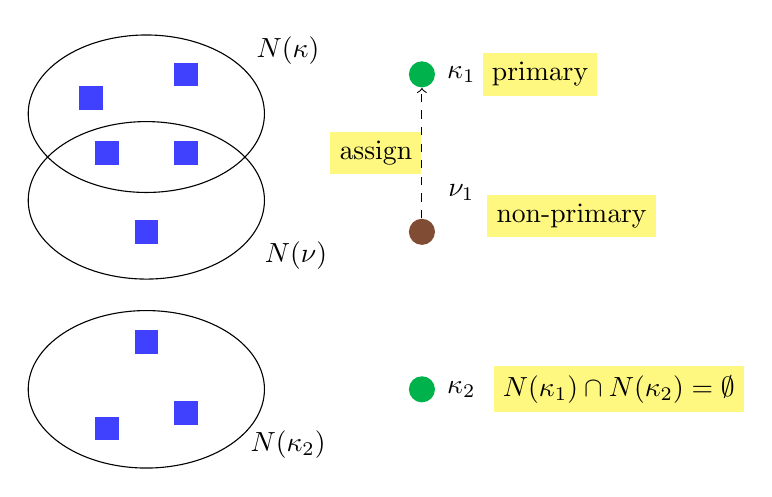
\begin{tikzpicture}[auto,every text node part/.style={align=center}]

\definecolor{primcolor}{rgb}{0,0.7,0.3}
\definecolor{nonprimcolor}{rgb}{0.5,0.3,0.2}

    %% primary demands
    \node[circle, fill=primcolor,  minimum size=.3cm] (kappa1) at (3.5, 8) {};
    \node (kappa1label) at (4,8) {$\kappa_1$};
    \node[draw, ellipse, minimum width=3cm, minimum height=2cm] (k1) at (0,7.5) {};
    \node[fill=blue!75, minimum size=.3cm] (mu1) at (-.7,7.7) {};
    \node[fill=blue!75, minimum size=.3cm] (mu2) at (.5,8) {};
    \node[fill=blue!75, minimum size=.3cm] (mu3) at (-.5,7) {};
    \node[fill=blue!75, minimum size=.3cm] (mu4) at (.5,7) {};
    \node (nbk) at (1.8,8.3) {$N(\kappa)$};
    \node[fill=yellow!50] (primary) at (5,8) {primary};

     % non-primary demands
    \node[circle, fill=nonprimcolor,  minimum size=.3cm] (nu) at (3.5, 6) {};
    \node (sib1label) at (4,6.5) {$\nu_1$};
    \node[fill=yellow!50] (nonprimary) at (5.4,6.2) {non-primary};

    \node[fill=blue!75, minimum size=.3cm] (mu5) at (0,6) {};

    \node[draw, ellipse, minimum width=3cm, minimum height=2cm] (k1) at (0,6.4) {};

    \node (nbnu1) at (1.9,5.7) {$N(\nu)$};

    % assignment
    \draw[->,dashed] (nu) to node[fill=yellow!50] {assign} (kappa1); 

    % primary kappa2
    \node (kappa2label) at (4,4) {$\kappa_2$};
    \node[fill=blue!75, minimum size=.3cm] (mu8) at (0,4.6) {};
    \node[fill=blue!75, minimum size=.3cm] (mu9) at (.5,3.7) {};
    \node[fill=blue!75, minimum size=.3cm] (mu10) at (-.5,3.5) {};
    \node (nbk2) at (1.8,3.3) {$N(\kappa_2)$};
    \node[draw, ellipse, minimum width=3cm, minimum height=2cm] (k1) at (0,4) {};
    \node[circle, fill=primcolor,  minimum size=.3cm] (kappa2) at (3.5, 4) {};
    \node[fill=yellow!50] (prop) at (6,4) {$N(\kappa_1)\cap N(\kappa_2) = \emptyset$};
  \end{tikzpicture}
\end{frame}

%%%%%%%%%%%%%%%%%%%%%%%%%%%%%%%%%%%%%%%%%%%%%%%%%%%%%%%%%%%%%%%%%%%%%%%%%%%%%%%%%%%%%%%%%%%%%%%%%%%%
%%% Neighborhood Structure for Siblings
%%%%%%%%%%%%%%%%%%%%%%%%%%%%%%%%%%%%%%%%%%%%%%%%%%%%%%%%%%%%%%%%%%%%%%%%%%%%%%%%%%%%%%%%%%%%%%%%%%%%

\begin{frame}
  \frametitle{Neighborhood Structure for Siblings}
  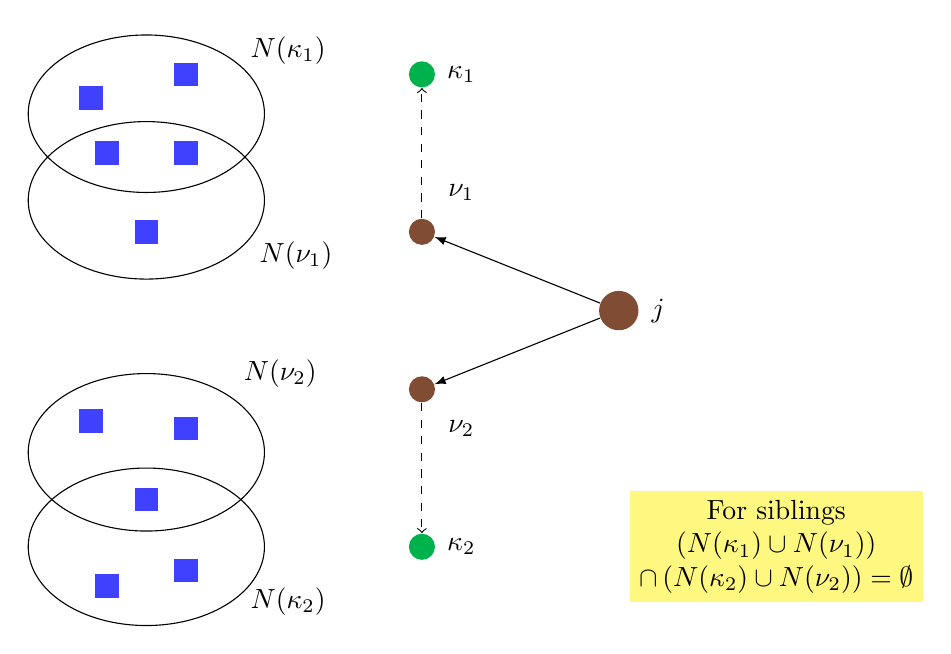
\begin{tikzpicture}[auto,every text node part/.style={align=center}]

\definecolor{primcolor}{rgb}{0,0.7,0.3}
\definecolor{nonprimcolor}{rgb}{0.5,0.3,0.2}

    \node[circle, fill=nonprimcolor, minimum size=.5cm] (client1) at (6, 5) {};
	% non-primary demands
    \node[circle, fill=nonprimcolor,  minimum size=.3cm] (nu1) at (3.5, 6) {};
    \node (sib1label) at (4,6.5) {$\nu_1$};
    \node[circle, fill=nonprimcolor,  minimum size=.3cm] (nu2) at (3.5, 4) {};
    \node (sib1label) at (4,3.5) {$\nu_2$};

    \node[draw, ellipse, minimum width=3cm, minimum height=2cm] (k1) at (0,6.4) {};
    \node[draw, ellipse, minimum width=3cm, minimum height=2cm] (k1) at (0,3.2) {};

    \node[fill=blue!75, minimum size=.3cm] (mu3) at (-.5,7) {};
    \node[fill=blue!75, minimum size=.3cm] (mu4) at (.5,7) {};

    \node[fill=blue!75, minimum size=.3cm] (mu5) at (0,6) {};
    \node[fill=blue!75, minimum size=.3cm] (mu6) at (-.7,3.6) {};
    \node[fill=blue!75, minimum size=.3cm] (mu7) at (.5,3.5) {};
    \node[fill=blue!75, minimum size=.3cm] (mu8) at (0,2.6) {};

    \node (nbnu1) at (1.9,5.7) {$N(\nu_1)$};
    \node (nbnu2) at (1.7,4.2) {$N(\nu_2)$};

    \node (clientlabel) at (6.5,5) {$j$};

    \draw[->,>=latex] (client1) -- (nu1);
    \draw[->,>=latex] (client1) -- (nu2);

    %% primary demands
    \pause
    \node[circle, fill=primcolor,  minimum size=.3cm] (kappa1) at (3.5, 8) {};
    \node (kappa1label) at (4,8) {$\kappa_1$};
    \node[draw, ellipse, minimum width=3cm, minimum height=2cm] (k1) at (0,7.5) {};
    \node[circle, fill=primcolor,  minimum size=.3cm] (kappa2) at (3.5, 2) {};
    \node (kappa2label) at (4,2) {$\kappa_2$};
    \node[draw, ellipse, minimum width=3cm, minimum height=2cm] (k1) at (0,2) {};
    \node[fill=blue!75, minimum size=.3cm] (mu1) at (-.7,7.7) {};
    \node[fill=blue!75, minimum size=.3cm] (mu2) at (.5,8) {};
    \node[fill=blue!75, minimum size=.3cm] (mu9) at (.5,1.7) {};
    \node[fill=blue!75, minimum size=.3cm] (mu10) at (-.5,1.5) {};
    \node (nbk1) at (1.8,8.3) {$N(\kappa_1)$};
    \node (nbk2) at (1.8,1.3) {$N(\kappa_2)$};

    % assignment
    \draw[->,dashed] (nu1) -- (kappa1); 
    \draw[->,dashed] (nu2) -- (kappa2);

    \node[fill=yellow!50] (prop) at (8,2) {For siblings \\
						$\left(N(\kappa_1) \cup N(\nu_1)\right)$ \\ 
						$ \cap \left(N(\kappa_2) \cup N(\nu_2)\right) =\emptyset$};

  \end{tikzpicture}
\end{frame}

%%%%%%%%%%%%%%%%%%%%%%%%%%%%%%%%%%%%%%%%%%%%%%%%%%%%%%%%%%%%%%%%%%%%%%%%%%%%%%%%%%%%%%%%%%%%%%%%%%%%
%%% Partitioning Example
%%%%%%%%%%%%%%%%%%%%%%%%%%%%%%%%%%%%%%%%%%%%%%%%%%%%%%%%%%%%%%%%%%%%%%%%%%%%%%%%%%%%%%%%%%%%%%%%%%%%

\begin{frame}
  \frametitle{Example of Partitioning}

  \begin{minipage}{.45\linewidth}
  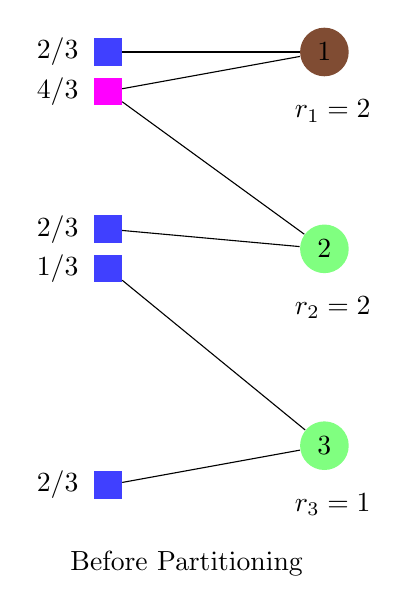
\begin{tikzpicture}[scale=0.5]
	
    \definecolor{primcolor}{rgb}{0,0.7,0.3}
    \definecolor{nonprimcolor}{rgb}{0.5,0.3,0.2}	

    \node[fill=blue!75,minimum size=.35cm] (fac31) at (.5,1) {};
    \node[left] (faclabel31) at (0,1) {$2/3$};

    \node[fill=blue!75,minimum size=.35cm] (fac21) at (.5,6.5) {};
    \node[fill=blue!75,minimum size=.35cm] (fac22) at (.5,7.5) {};

    % label
    \node[left] (faclabel21) at (0,6.5) {$1/3$};
    \node[left] (faclabel22) at (0,7.5) {$2/3$};

    \node[fill=Fuchsia,minimum size=.35cm] (fac11) at (.5,11) {};
    \node[fill=blue!75,minimum size=.35cm] (fac12) at (.5,12) {};

    % label
    \node[left] (faclabel11) at (0,11) {$4/3$};
    \node[left] (faclabel12) at (0,12) {$2/3$};

    \node[circle,fill=green!50] (client3) at (6,2) {$3$};
    \node[circle,fill=green!50] (client2) at (6,7) {$2$};
    \node[circle,fill=nonprimcolor] (client1) at (6,12) {$1$};

    \node[right] (demand3) at (5,.5) {$r_3=1$};
    \node[right] (demand2) at (5,5.5) {$r_2=2$};
    \node[right] (demand1) at (5,10.5) {$r_1=2$};
  
    \foreach \from/\to in {fac31/client3,fac21/client3,fac22/client2,fac11/client2,fac11/client1,fac12/client1}
    \draw (\from)--(\to);

    \node at (2.5,-1) {Before Partitioning};
  \end{tikzpicture}
  \end{minipage}
  \pause
  \begin{minipage}{.45\linewidth}
    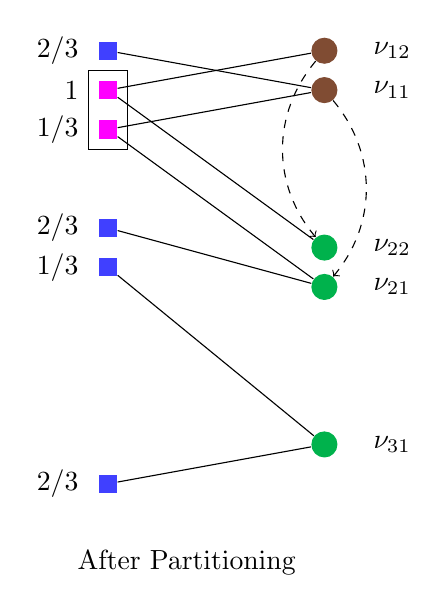
\begin{tikzpicture}[scale=0.5,decoration=snake]
	
	\definecolor{primcolor}{rgb}{0,0.7,0.3}
	\definecolor{nonprimcolor}{rgb}{0.5,0.3,0.2}
	
	% facilities
    \node[fill=blue!75,minimum size=.15cm] (fac31) at (.5,1) {};
    \node[fill=blue!75,minimum size=.15cm] (fac21) at (.5,6.5) {};
    \node[fill=blue!75,minimum size=.15cm] (fac22) at (.5,7.5) {};
    \node[fill=Fuchsia,minimum size=.15cm] (fac11) at (.5,10) {};
    \node[fill=Fuchsia,minimum size=.15cm] (fac12) at (.5,11) {};
    \node[fill=blue!75,minimum size=.15cm] (fac13) at (.5,12) {};

 	\node[left] (faclabel31) at (0,1) {$2/3$};
    \node[left] (faclabel21) at (0,6.5) {$1/3$};
    \node[left] (faclabel22) at (0,7.5) {$2/3$};
    \node[left] (faclabel11) at (0,10) {$1/3$};
    \node[left] (faclabel12) at (0,11) {$1$};
    \node[left] (faclabel13) at (0,12) {$2/3$};

	% demands
    \node[circle,fill=primcolor,minimum size=.2cm] (client31) at (6,2) {};
    \node[circle,fill=primcolor,minimum size=.2cm] (client21) at (6,6) {};
    \node[circle,fill=primcolor,minimum size=.2cm] (client22) at (6,7) {};
    \node[circle,fill=nonprimcolor,minimum size=.2cm] (client11) at (6,11) {};
    \node[circle,fill=nonprimcolor,minimum size=.2cm] (client12) at (6,12) {};

    \node[right] (demand31) at (7,2) {$\nu_{31}$};
    \node[right] (demand21) at (7,6) {$\nu_{21}$};
    \node[right] (demand22) at (7,7) {$\nu_{22}$};
    \node[right] (demand11) at (7,11) {$\nu_{11}$};
    \node[right] (demand12) at (7,12) {$\nu_{12}$};

    \foreach \from/\to in {fac31/client31,fac21/client31,fac22/client21,fac11/client21,fac12/client22,fac11/client11,fac13/client11,fac12/client12}
    \draw (\from)--(\to);

    \node at (2.5,-1) {After Partitioning};

    %% for split
    \draw (0, 9.5) rectangle (1, 11.5);

    %\pause

    \path[->,dashed] (client12) edge[bend right=40] (client22);
    \path[->,dashed] (client11) edge[bend left=40] (client21);
  \end{tikzpicture}
      
\end{minipage}
\end{frame}

%%%%%%%%%%%%%%%%%%%%%%%%%%%%%%%%%%%%%%%%%%%%%%%%%%%%%%%%%%%%%%%%%%%%%%%%%%%%%%%%%%%%%%%%%%%%%%%%%%%%
%%% Summary of Partition Properties
%%%%%%%%%%%%%%%%%%%%%%%%%%%%%%%%%%%%%%%%%%%%%%%%%%%%%%%%%%%%%%%%%%%%%%%%%%%%%%%%%%%%%%%%%%%%%%%%%%%%

\begin{frame}
  \frametitle{Summary of Partitioning}

  \begin{columns}[T]
    \column{0.5\textwidth} 
    \textcolor{blue}{Partitioning:}
    \begin{itemize}\addtolength{\itemsep}{0.5\baselineskip}
	\item Clients $\rightarrow$ demands
	\item Sites $\rightarrow$ facilities

	\item $(x^\ast,y^\ast)$ $\rightarrow (\barx,\bary)$
	\item $\sum_{\mu}\barx_{\mu\nu} = 1$
	\item $\barx_{\mu\nu} = \bary_\mu$ or $0$
        \end{itemize}

    \column{0.5\textwidth}
    \textcolor{blue}{Structure:}
    \begin{itemize}

    \item If $\kappa_1,\kappa_2$ primary then
      $N(\kappa_1)\cap N(\kappa_2) = \emptyset$
    \begin{block}<2->{}
      small facility cost
    \end{block}
  \item Each non-primary $\nu$ assigned to $\kappa$ with
	\begin{itemize}
        \item $N(\kappa)\cap N(\nu) \neq \emptyset$
	\item priority$(\kappa)$ $\le$ priority $(\nu)$
        \end{itemize}
        \begin{block}<3->{}
          small connection cost of $\nu$
        \end{block}
  \item $N(\kappa_1) \cup N(\nu_1)\;\cap\;N(\kappa_2) \cup N(\nu_2) = \emptyset$
    \begin{block}<4->{}
      fault-tolerance
    \end{block}
  \end{itemize}
\end{columns}
\end{frame}




%%%%%%%%%%%%%%%%%%%%%%%%%%%%%%%%%%%%%%%%%%%%%%%%%%%%%%%%%
%% Partition Implementation
%%%%%%%%%%%%%%%%%%%%%%%%%%%%%%%%%%%%%%%%%%%%%%%%%%%%%%%%%
%%
\begin{frame}
  \frametitle{Partition Implementation}

  \Large{\textcolor{blue}{Partition implementation: two phases}}

  \vspace{.3in}
  \begin{itemize}\addtolength{\itemsep}{1\baselineskip}
  \item \large{Phase 1, the partitioning phase}
    \begin{itemize}
    \item Define demands
    \item Allocate facilities
    \end{itemize}
  \item \large{Phase 2, the augmenting phase}
    \begin{itemize}
    \item Add facilities to make neighborhood unit
    \end{itemize}
  \end{itemize}
\end{frame}

\begin{frame}
  \frametitle{Phase 1, Step 1} 
  \setbeamercovered{invisible}

        \setbeamercolor{postit}{fg=blue,bg=yellow}
        \begin{beamercolorbox}[sep=.5em,wd=10cm]{postit}
          For each client, arrange neighbor facilities near
          to far
        \end{beamercolorbox}
  
  \begin{center}
  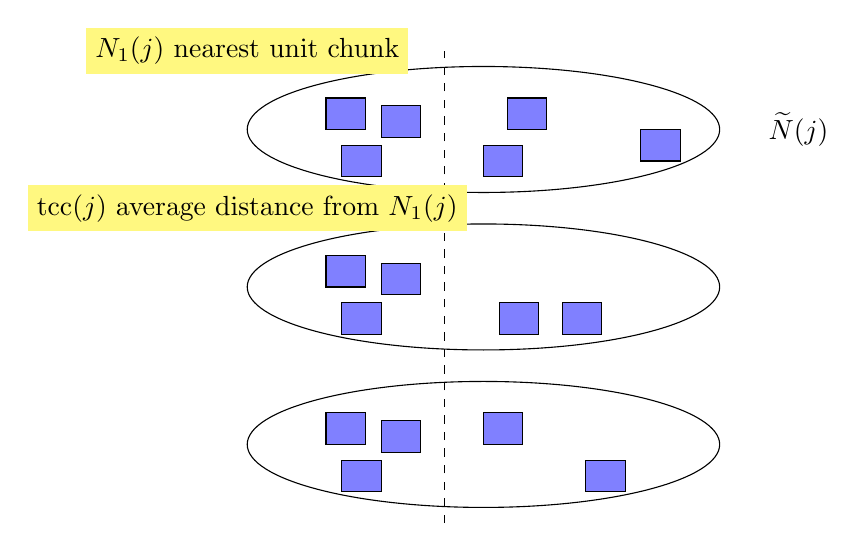
\begin{tikzpicture}
    \node (label2) at (4,4) {$\wtildeN(j)$};

    \draw (0,0) ellipse (3cm and .8cm);
    \draw (0,2) ellipse (3cm and .8cm);
    \draw (0,4) ellipse (3cm and .8cm);


    %% squares, facilities
    \draw[fill=blue!50] (-1.5,0) rectangle (-2,.4);
    \draw[fill=blue!50] (-.8,-.1) rectangle (-1.3,.3);
    \draw[fill=blue!50] (-1.3,-.2) rectangle (-1.8,-.6);

    \draw[fill=blue!50] (0,0) rectangle (.5,.4);
    \draw[fill=blue!50] (1.3,-.2) rectangle (1.8,-.6);
         
    \draw[fill=blue!50] (-1.5,2) rectangle (-2,2.4);
    \draw[fill=blue!50] (-.8,1.9) rectangle (-1.3,2.3);
    \draw[fill=blue!50] (-1.3,1.8) rectangle (-1.8,1.4);

    \draw[fill=blue!50] (.2,1.8) rectangle (.7,1.4);
    \draw[fill=blue!50] (1,1.8) rectangle (1.5,1.4);

    \draw[fill=blue!50] (-1.5,4) rectangle (-2,4.4);
    \draw[fill=blue!50] (-.8,3.9) rectangle (-1.3,4.3);
    \draw[fill=blue!50] (-1.3,3.8) rectangle (-1.8,3.4);

    \draw[fill=blue!50] (0,3.4) rectangle (.5,3.8);
    \draw[fill=blue!50] (.3,4) rectangle (.8,4.4);
    \draw[fill=blue!50] (2,3.6) rectangle (2.5,4);

    \pause
    \draw[style=dashed] (-.5,-1) -- (-.5,5);
    \node[fill=yellow!50] (label1) at (-3,5) {$N_1(j)$ nearest unit chunk};
    \node[fill=yellow!50] (tcc) at (-3,3) {$\tcc(j)$ average distance from $N_1(j)$};
  \end{tikzpicture}
  \end{center}
\end{frame}

\begin{frame}
  \frametitle{Phase 1, Step 2} 
        \setbeamercolor{postit}{fg=blue,bg=yellow}
        \begin{beamercolorbox}[sep=.5em,wd=10cm]{postit}
          Select client $p$ with $\min \tcc(p) + \alpha_p^\ast$.
          Two cases:
        \end{beamercolorbox}

        \begin{columns}[b]
          \column{0.5\textwidth}
          \begin{center}
          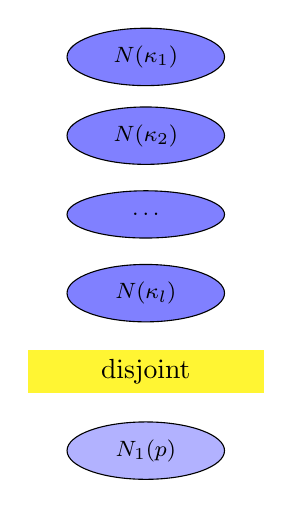
\begin{tikzpicture}
            \node[fill=blue!50,draw,ellipse,minimum width=2cm,minimum height=.6cm] at (0,0) {\footnotesize{$N(\kappa_1)$}};
            \node[fill=blue!50,draw,ellipse,minimum width=2cm,minimum height=.6cm] at (0,-1) {\footnotesize{$N(\kappa_2)$}};
            \node[fill=blue!50,draw,ellipse,minimum width=2cm,minimum height=.6cm] at (0,-2) {\footnotesize{$\ldots$}};
            \node[fill=blue!50,draw,ellipse,minimum width=2cm,minimum height=.6cm] at (0,-3) {\footnotesize{$N(\kappa_l)$}};

            \node[fill=blue!30,draw,ellipse,minimum width=2cm,minimum height=.6cm] at (0,-5) {\footnotesize{$N_1(p)$}};

            \node[fill=yellow!80,minimum width=3cm] at (0,-4) {disjoint};
          \end{tikzpicture}
          \textcolor{blue}{Case 1}
          \end{center}
          %
          \column{0.5\textwidth}
          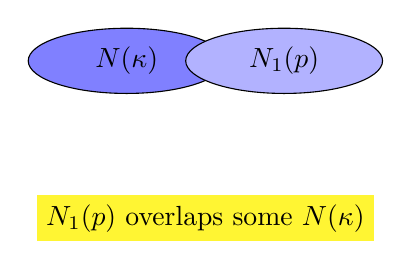
\begin{tikzpicture}
            \node[fill=blue!50,draw,ellipse,minimum width=2.5cm,minimum height=.6cm] at (0,0) {$N(\kappa)$};
            \node[fill=blue!30,draw,ellipse,minimum width=2.5cm,minimum height=.6cm] at (2,0) {$N_1(p)$};
            \node[fill=yellow!80] at (1,-2) {$N_1(p)$ overlaps some $N(\kappa)$};
          \end{tikzpicture}
          \textcolor{blue}{Case 2}
        \end{columns}
\end{frame}

%%% make a new primary
\begin{frame}
  \frametitle{Phase 1, Step 2 (Cont. Case 1)}
  \begin{center}
  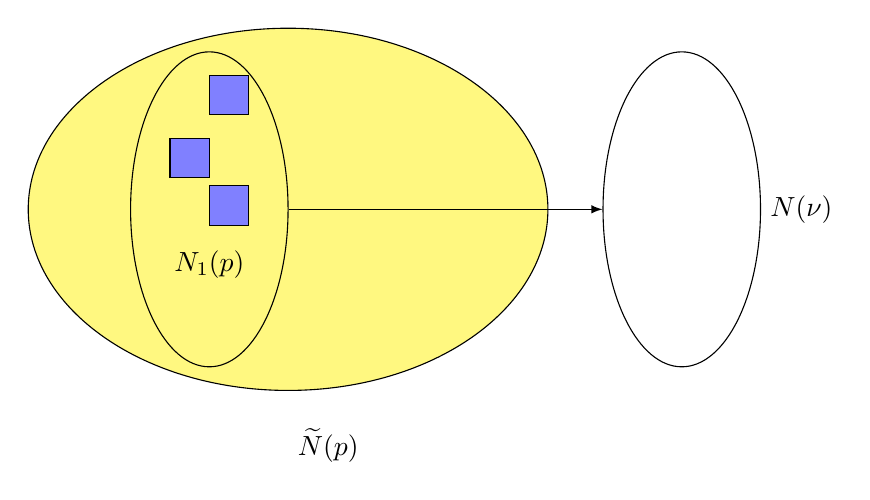
\begin{tikzpicture}
    \draw[fill=yellow!50] (0,0) ellipse (3.3cm and 2.3cm);
    \node[right] at (0,-3) {$\wtildeN(p)$};
    
    \node[draw,fill=yellow!50,ellipse,minimum width=2cm,minimum height=4cm] (chunkone) at (-1,0) {};
    \node[above] at (-1,-1) {$N_1(p)$};
    
    \draw[fill=blue!50] (-1,1.2) rectangle (-.5,1.7);
    \draw[fill=blue!50] (-1.5,0.4) rectangle (-1,.9);
    \draw[fill=blue!50] (-1,-0.2) rectangle (-.5,.3);

    \node[draw,ellipse,minimum width=2cm,minimum height=4cm] (neighbornu) at (5,0) {};
    \node[right] at (6,0) {$N(\nu)$};

    \draw[->,>=latex] (chunkone) -- (neighbornu);
  \end{tikzpicture}
  \end{center}
\end{frame}

\begin{frame}
  \frametitle{Phase 1, Step 2 (Case 1)}
        \setbeamercolor{postit}{fg=blue,bg=yellow}
        \begin{beamercolorbox}[sep=.5em,wd=10cm]{postit}
          All facilities in $N_1(p)$ moved to $N(\nu)$
        \end{beamercolorbox}

  \vspace{1cm}
  \begin{center}
  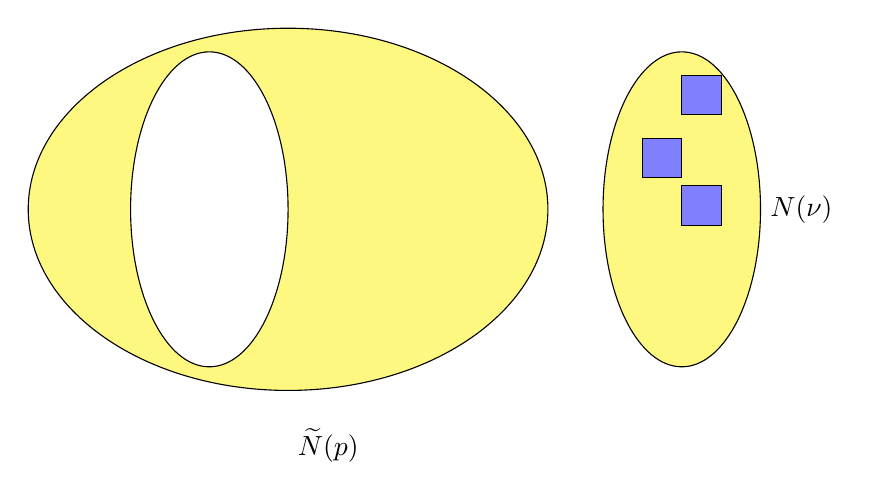
\begin{tikzpicture}
    \draw[fill=yellow!50] (0,0) ellipse (3.3cm and 2.3cm);
    \node[right] at (0,-3) {$\wtildeN(p)$};
    
    \draw[fill=white] (-1,0) ellipse (1cm and 2cm);
    
    \draw[fill=yellow!50] (5,0) ellipse (1cm and 2cm);
    \node[right] at (6,0) {$N(\nu)$};

    \draw[fill=blue!50] (5,1.2) rectangle (5.5,1.7);
    \draw[fill=blue!50] (4.5,.4) rectangle (5,.9);
    \draw[fill=blue!50] (5,-.2) rectangle (5.5,.3);

  \end{tikzpicture}
  \end{center}
\end{frame}

%%% intersect with a primary
\begin{frame}
  \frametitle{Phase 1, Step 2 (Cont. Case 2)}

  Move all overlapping facilities in $\wtildeN(p) \cap
  N(\kappa)$ into $N(\nu)$.

  \vspace{.5cm}
  \begin{center}
  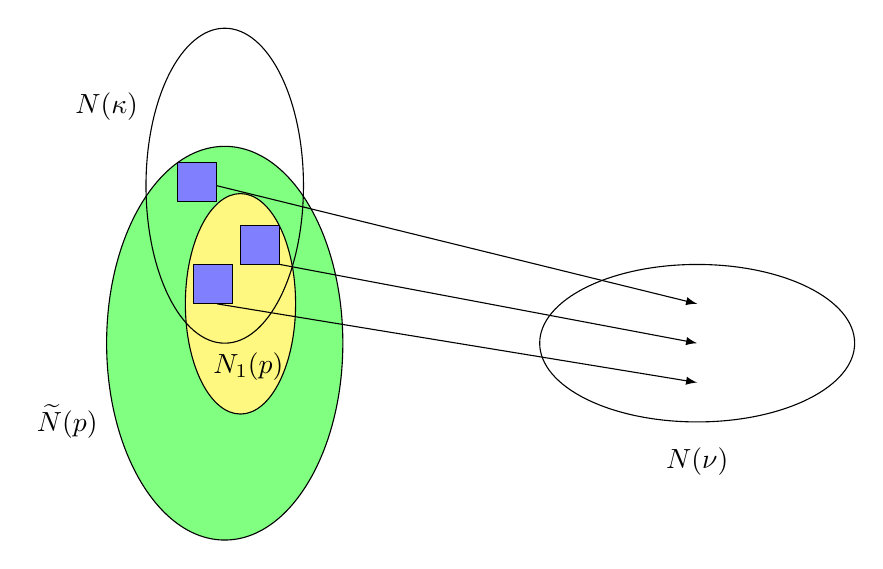
\begin{tikzpicture}
  \draw[fill=green!50] (1,1) ellipse (1.5cm and 2.5cm);
  \node (client) at (-1,0) {$\wtildeN(p)$};

  \draw[fill=yellow!50] (1.2,1.5) ellipse (.7cm and 1.4cm);
  \node (prefix) at (1.3,.7) {$N_1(p)$};

  \draw (1,3) ellipse (1cm and 2cm);
  \node (primary) at (-.5,4) {$N(\kappa)$};

  \draw (7,1) ellipse (2cm and 1cm);
  \node (demand) at (7,-.5) {$N(\nu)$};

  %% fac
  \draw[fill=blue!50] (1.2,2) rectangle (1.7,2.5);
  \draw[fill=blue!50] (.4,2.8) rectangle (.9,3.3);
  \draw[fill=blue!50] (.6,1.5) rectangle (1.1,2);

  \draw [->,>=latex] (1.7,2) -- (7,1);
  \draw [->,>=latex] (.9,3) -- (7,1.5);
  \draw [->,>=latex] (.9,1.5) -- (7,.5);
  \end{tikzpicture}
  \end{center}
\end{frame}

\begin{frame}
  \frametitle{Phase 2}

  \setbeamercolor{postit}{fg=blue,bg=yellow}
  \begin{beamercolorbox}[sep=.5em,wd=10cm]{postit}
    Add facilities from $\wtildeN(j)$ to $N(\nu)$ until
    total connection value is $1$.
  \end{beamercolorbox}

  \vspace{1cm}
  \begin{center}
  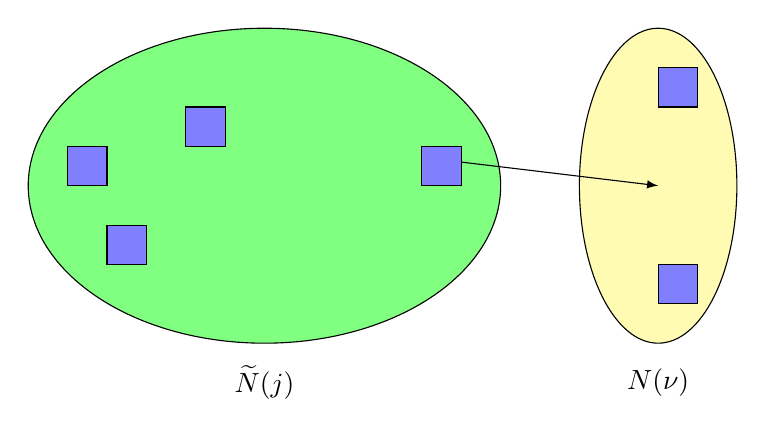
\begin{tikzpicture}
    \draw[fill=green!50] (0,0) ellipse (3cm and 2cm);
    \node (label1) at (0,-2.5) {$\wtildeN(j)$};

    \draw[fill=yellow!30] (5,0) ellipse (1cm and 2cm);
    \node (label2) at (5,-2.5) {$N(\nu)$};

    \draw[fill=blue!50] (-2.5,0) rectangle (-2,.5);
    \draw[fill=blue!50] (-2,-1) rectangle (-1.5,-.5);
    \draw[fill=blue!50] (-1,.5) rectangle (-.5,1);
    \draw[fill=blue!50] (2,0) rectangle (2.5,.5);

    \draw[fill=blue!50] (5,1) rectangle (5.5,1.5);
    \draw[fill=blue!50] (5,-1.5) rectangle (5.5,-1);

    \draw [->,>=latex] (2.5,.3) -- (5,0);
  \end{tikzpicture}
  \end{center}

\end{frame}

\begin{frame}
  \begin{block}{}
    \large{
    We are done with adaptive partitioning and got a structured fractional solution
    }
  \end{block}
  \vspace{.5in}
  \begin{block}{}
    \Large{
      \textcolor{blue}{
    Next: the rounding algorithms...
    }
    }
  \end{block}
\end{frame}
\section[Algorithms]{Approximation Algorithms}
%%
%% 3.3 Rounding: fault-tolerant made easy, all ratios preserved
%%     the 1.575 rounding is subtle
\subsection[Rounding]{LP-rounding Algorithms}
%%%%%%%%%%%%%%%%%%%%%%%%%%%%%%%%%%%%%%%%%%%%%%%%%%%%%%%%%%%%%%%%%%%%%%%%%%%%%%%%%%%%%%%%%%%%%%%%%%%%
%%% 3-Approximation
%%%%%%%%%%%%%%%%%%%%%%%%%%%%%%%%%%%%%%%%%%%%%%%%%%%%%%%%%%%%%%%%%%%%%%%%%%%%%%%%%%%%%%%%%%%%%%%%%%%%

\begin{frame}
  \frametitle{$3$-Approximation for FTFP}

{\large

\textcolor{blue}{Client priority values}	
	
	\begin{itemize}
		\item $\tcc(j) + \alpha_j^\ast$
		\\
		{\normalsize \textcolor{gray}{(average connection cost + dual value)}}
	\end{itemize}
	
\textcolor{blue}{Rounding}

  	\begin{itemize}
  	\item \textcolor{Sepia}{Facilities:}
 					Each primary $\kappa$ opens random $\mu\in N(\kappa)$
  	\item \textcolor{Sepia}{Connections:}
 					All demands assigned to $\kappa$ connect to $\mu$
  	\end{itemize}

\textcolor{blue}{Analysis}

  \begin{itemize}
  	\item \textcolor{Sepia}{Fault-Tolerance:}
 			$\nu$ uses only facilities in $N(\nu) \cup N(\kappa)$
  	\item \textcolor{Sepia}{Cost:} $\le 3\cdot\LP^\ast$, because
    	\begin{itemize}
    		\item Facility cost $\le F^\ast$
    		\item Connection cost $\le C^\ast + 2\cdot\LP^\ast$
    	\end{itemize}
 	\end{itemize}
}
\end{frame}

%%%%%%%%%%%%%%%%%%%%%%%%%%%%%%%%%%%%%%%%%%%%%%%%%%%%%%%%%%%%%%%%%%%%%%%%%%%%%%%%%%%%%%%%%%%%%%%%%%%%
%%% 1+2/e Approximation
%%%%%%%%%%%%%%%%%%%%%%%%%%%%%%%%%%%%%%%%%%%%%%%%%%%%%%%%%%%%%%%%%%%%%%%%%%%%%%%%%%%%%%%%%%%%%%%%%%%%

\begin{frame}
  \frametitle{$1.736$-Approximation for FTFP} 

{\large

\textcolor{blue}{Client priority values}	
	
	\begin{itemize}
		\item $\tcc(j) + \alpha_j^\ast$ 
			\\
				{\normalsize \textcolor{gray}{(average connection cost + dual value)}}
	\end{itemize}

\textcolor{blue}{Rounding}

  	\begin{itemize}
  	  	\item  \textcolor{Sepia}{Facilities:} 
			\begin{itemize}
				\item Each primary $\kappa$ opens random $\mu\in N(\kappa)$
				\item Other facilities open randomly independently
			\end{itemize}
	  	\item \textcolor{Sepia}{Connections:} 
	 		\begin{itemize}
					\item if a neighbor open, connect to nearest neighbor
					\item else, connect via assigned primary demand
			\end{itemize}
  	\end{itemize}

\textcolor{blue}{Analysis}

  \begin{itemize}
  	\item \textcolor{Sepia}{Fault-Tolerance:} $\nu$ uses only facilities in
    			$N(\nu) \cup N(\kappa)$
  	\item \textcolor{Sepia}{Cost:} $\le (1+2/e)\,\LP^\ast$, because
    	\begin{itemize}
    		\item Facility cost $\le F^\ast$
    		\item Connection cost $\le C^\ast + \frac{2}{e}\cdot \LP^\ast$
    	\end{itemize}
  \end{itemize}
}
\end{frame}

%%%%%%%%%%%%%%%%%%%%%%%%%%%%%%%%%%%%%%%%%%%%%%%%%%%%%%%%%%%%%%%%%%%%%%%%%%%%%%%%%%%%%%%%%%%%%%%%%%%%
%%% 1.575-approx
%%%%%%%%%%%%%%%%%%%%%%%%%%%%%%%%%%%%%%%%%%%%%%%%%%%%%%%%%%%%%%%%%%%%%%%%%%%%%%%%%%%%%%%%%%%%%%%%%%%%

\begin{frame}
  \frametitle{$1.575$-Approximation for FTFP -- Idea}


{\textcolor{blue}{More intricate neighborhood structure}}
    \begin{itemize}
    	\item Two neighborhoods: close and far, $N(\nu)= N_{\cls}(\nu) \cup N_{\far}(\nu)$
		\item $N_{\cls}(\nu)=$ nearest $(1/\gamma)$-fraction of $N(\nu)$
  		\item $N_{\cls}(\nu)\cap N_{\cls}(\kappa) \neq\emptyset$, if $\nu$ assigned to $\kappa$
  		\item For siblings $\nu_1, \nu_2$, $N_{\cls}(\kappa_1) \cup
    			N(\nu_1)$ and $N_{\cls}(\kappa_2) \cup N(\nu_2)$ disjoint
				\item ...
    \end{itemize}

	\begin{center}
	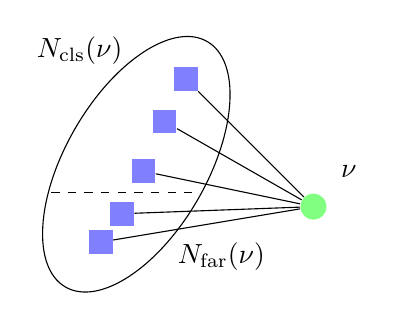
\begin{tikzpicture}[scale = 0.9,align = right]
    \node[fill=blue!50,rectangle,minimum size=.3cm] (mu1) at (1,1.5) {};
    \node[fill=blue!50,rectangle,minimum size=.3cm] (mu2) at (1.3,1.9) {};      
	\node[fill=blue!50,rectangle,minimum size=.3cm] (mu3)  at (1.6,2.5) {};      
	\node[fill=blue!50,rectangle,minimum size=.3cm] (mu4) at (1.9,3.2) {};     
	\node[fill=blue!50,rectangle,minimum size=.3cm] (mu5) at (2.2,3.8) {};      
    \draw[rotate=-30] (0,3) ellipse (1 and 2);
 \draw[dashed] (0.3,2.2) -- (2.3,2.2);
    \node[fill=green!50,circle,minimum size=.3cm] (nu) at (4,2) {};
    \node at (4.5,2.5) {$\nu$};

    \node at (.7,4.2) {$N_{\cls}(\nu)$};
    \node at (2.7,1.3) {$N_{\far}(\nu)$};

    \foreach \from in {mu1,mu2,mu3,mu4,mu5}
    \draw (\from) -- (nu);
  \end{tikzpicture}
\end{center}

\end{frame}

%%%%%%%%%%%%%%%%%%%%%%%%%%%%%%%%%%%%%%%%%%%%%%%%%%%%%%%%%%%%%%%%%%%%%%%%%%%%%%%%%%%%%%%%%%%%%%%%%%%%

%%% 1+2/e approx
\begin{frame}
\frametitle{$1.575$-Approximation for FTFP}

{\large

\textcolor{blue}{Client priority values}	
	
	\begin{itemize}
		\item $\tcccls(j) + \dmaxcls(j)$
			\\
			{\normalsize \textcolor{gray}{(average + worst connection cost to close neighborhood)}}
	\end{itemize}

\textcolor{blue}{Rounding (extension of Byrka's)}

  	\begin{itemize}
  	  	\item  \textcolor{Sepia}{Facilities:} 
			\begin{itemize}
				\item Each primary $\kappa$ opens random $\mu\in N_{\cls}(\kappa)$
				\item Other facilities open randomly independently
			\end{itemize}
	  	\item \textcolor{Sepia}{Connections:} 
	 		\begin{itemize}
					\item if a neighbor open, connect to nearest neighbor
					\item else, connect via assigned primary demand
			\end{itemize}
  	\end{itemize}

\textcolor{blue}{Analysis}

  \begin{itemize}
  	\item \textcolor{Sepia}{Fault-Tolerance:} $\nu$ uses only facilities in
	    $N(\nu) \cup N_{\cls}(\kappa)$
	
  	\item \textcolor{Sepia}{Cost:} $\le \gamma\cdot\LP$ for $\gamma = 1.575$, because
    \begin{itemize}
    \item Facility cost $ \leq \gamma\cdot F^\ast$
    \item Connection cost $ \leq \gamma\cdot C^\ast$
    \end{itemize}
\end{itemize}
}

\end{frame}


%%%%%%%%%%%%%%%%%%%%%%%%%%%%%%%%%%%%%%%%%%%%%%%%%%%%%%%%%%%%%%%%%%%%%%%%%%%%%%%%%%%%%%%%%%%%%%%%%%%%
\subsection[Dual-fitting]{Greedy Algorithm and Analysis}
%% 3.4 Greedy, Dual-fitting, and hard example for local-charging
\begin{frame}
  \frametitle{Greedy and Dual-fitting}
  \begin{itemize}\addtolength{\itemsep}{1\baselineskip}
  \item Greedy in polynomial time
    \begin{itemize}
    \item Best star can be found quickly
    \item Best star remains best
    \end{itemize}
  \item Ratio $H_n$ (Wolsey's result):
    Greedy is $H_n$-approx for
    \begin{itemize}
    \item Minimizing a linear function
    \item Subject to submodular constraint
    \end{itemize}
  \item Lower bound $\Omega(\log n / \log\log n)$ for dual-fitting
    \begin{itemize}
    \item Example has $k$ groups, $n = k^k$
    \item Shrinking factor is $k/2$
    \end{itemize}
  \end{itemize}
\end{frame}

\begin{frame}{Dual-fitting Example}

    \color{blue}{Dual feasibility forces a ratio of $k/2$, number of clients $n=k^k$}
    \color{black}
  \begin{figure}
    \centering
    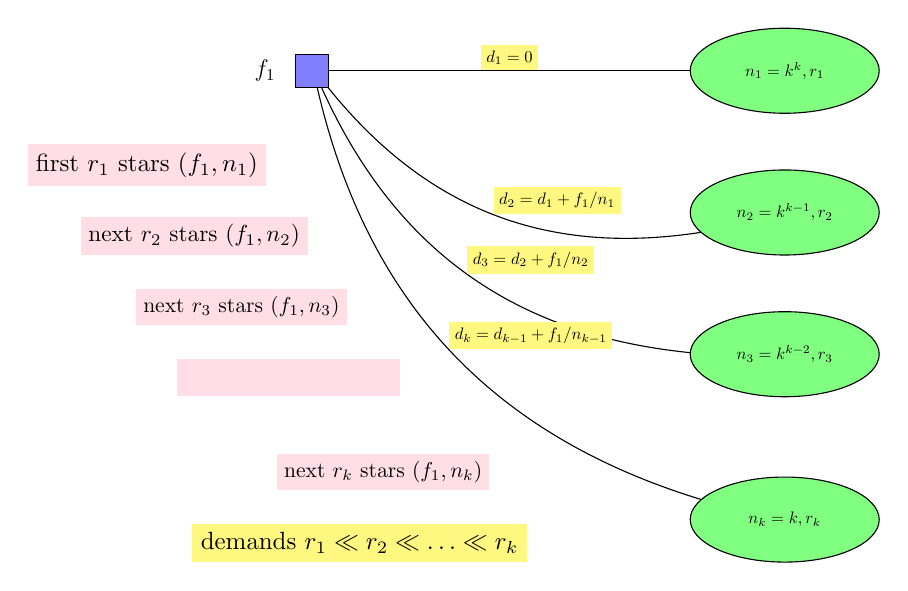
\begin{tikzpicture}[auto,scale=0.6, every node/.style={scale=0.6}]
    \node[draw,rectangle,minimum size=.7cm,fill=blue!50] (fac) at (-4,0) {};
    \node at (-5,0) {\Large{$f_1$}};
    
    \node[draw,ellipse,minimum width=4cm,minimum
    height=1.8cm,fill=green!50] (client1) at
    (6,0) {$n_1 = k^k, r_1$};
    \node[draw,ellipse,minimum width=4cm,minimum
    height=1.8cm,fill=green!50] (client2) at
    (6,-3) {$n_2 = k^{k-1}, r_2$};
    \node[draw,ellipse,minimum width=4cm,minimum
    height=1.8cm,fill=green!50] (client3) at
    (6,-6) {$n_3 = k^{k-2}, r_3$};
    \node[draw,ellipse,minimum width=4cm,minimum
    height=1.8cm,fill=green!50] (clientk) at
    (6,-9.5) {$n_k = k, r_k$};
    
    \node[fill=yellow!50,scale=1.5] at (-3,-10) {demands $r_1 \ll r_2 \ll \ldots \ll r_k$};

    \draw (fac) to node[fill=yellow!50] {$d_1=0$} (client1);
    \draw[bend right] (fac) to node[fill=yellow!50] {$d_2 = d_1 + f_1 /
      n_1$}  (client2);
    \draw[bend right] (fac) to node[fill=yellow!50] {$d_3 = d_2 + f_1 /
      n_2$}  (client3);
    \draw[bend right] (fac) to node[fill=yellow!50] {$d_k = d_{k-1} + f_1 / n_{k-1}$}  (clientk);

    \node[fill=Pink!50,scale=1.5] at (-7.5,-2) {first $r_1$ stars $(f_1,n_1)$};
    \node[fill=Pink!50,scale=1.4] at (-6.5,-3.5) {next $r_2$ stars $(f_1,n_2)$};
    \node[fill=Pink!50,scale=1.3] at (-5.5,-5) {next $r_3$ stars $(f_1,n_3)$};
    \node[fill=Pink!50,scale=1.2] at (-4.5,-6.5) {\color{Pink!50}\large{next $r_1$ stars $(f_1,n_1)$}};
    \node[fill=Pink!50,scale=1.3] at (-2.5,-8.5) {next $r_k$ stars $(f_1,n_k)$};
  \end{tikzpicture}
\end{figure}
\end{frame}


\section[End]{Summary}
%% 4. Open problems and future work
%%     - dual-fitting for FTFP
%%     - 1.463 for UFL
%%\begin{frame}
%%  \frametitle{Results for FTFP}
%%  \begin{itemize}
%%  \item \color{red}
%%    Q: Is there a simple reduction from FTFP to UFL?
%%  \item<2,8> \color{blue}
%%    A: Not sure, for the uniform demand case yes.
%%  \item \color{red}
%%    Q: Which one is easier, FTFP or FTFL?
%%  \item<3,8> \color{blue}
%%    A: FTFP. FTFP reduces to FTFL.
%%  \item \color{red}
%%    Q: Can FTFP have a better ratio than FTFL?
%%  \item<4,8> \color{blue}
%%    A: Yes, 1.575 matches UFL and beats 1.7245 for FTFL.
%%  \item \color{red}
%%    Q: When all $r_j$ are large, do you get a ratio $1$?
%%  \item<5,8> \color{blue}
%%    A: Yes, because of demand reduction.
%%  \item \color{red}
%%    Q: Does greedy have $O(1)$ ratio or not?
%%  \item<6,8> \color{blue}
%%    A: Maybe, but dual-fitting will not do.
%%  \item \color{red}
%%    Q: What is the best possible ratio for FTFP?
%%  \item<7,8> \color{blue}
%%    A: Likely to be 1.463, but not a sure thing.
%% \end{itemize}
%%\end{frame}

\begin{frame}
  \frametitle{Summary}
  
{\large
  {\textcolor{blue}{Results}}

  \begin{itemize}
  	\item $1.575$-approximation algorithm for FTFP
	\item Technique for extending LP-rounding algorithms for UFL to FTFP
  \end{itemize}

\vspace{0.2in}
\pause
  {\textcolor{blue}{Open Problems}}

  \begin{itemize}
  \item Can FTFL be approximated with the same ratio?
  \item LP-free algorithms for FTFP or FTFL with constant ratio?
  \item Close the $1.463-1.488$ gap for UFL!
  \end{itemize}
}

\end{frame}


\end{document}

